% METRIC SPACES NOTES
% OLIVER DIXON, 2023
%
% You can download the large cover image (to be named `cover.jpg') from:
% https://www-users.york.ac.uk/~od641/l5-notes/assets/ms-cover.jpg. You can
% request a (very large ~20MB) layer-rich XCF copy of the cover by e-mailing me.
%
% To compile this document in `draft' mode, which does not require many external
% assets, issue \drafttrue in place of \draftfalse. Do not distribute any
% generated draft copies!
%
% A note on PGF externalisation: due to the inevitable file-size increase
% incurred when importing external PDFs (with their own embedded fonts), the PGF
% external library is used as sparsely as possible, and only in cases where
% on-line point-sampling would cause significant slow-down, such as in cases of
% three-dimensional meshes (e.g. the global continuity diagram). In these cases,
% the tikzpicture environment should be encapsulated in a group with the
% external/export key set to true. The library is also known to clash with
% tcolorbox, for which a fix was proposed by the author of the latter:
% https://tex.stackexchange.com/a/497136

\documentclass{article}
\pdfsuppresswarningpagegroup=1
\newif\ifdraft
\drafttrue

\usepackage[
    a4paper,
    top=1.5in,
    bottom=1.5in,
    left=1in,
    right=1in,
]{geometry}
\usepackage[
    angle=90,
    hanchor=l,
    hpos=.05\paperwidth,
    fontsize=1.5em,
    color=black,
    firstpageonly,
    stamp=false
]{draftwatermark}
\usepackage[en-GB]{datetime2}
\usepackage[missing=master]{gitinfo2}
\usepackage[sorting=none, style=alphabetic, backend=biber]{biblatex}
\usepackage{fancyhdr, anyfontsize, amsthm, mathtools, amssymb, tcolorbox,
    lastpage, enumitem, tikz, multirow, pgfplots}
\usepackage[hypcap=false]{caption}
\usepackage[explicit]{titlesec}
\usepackage[colorlinks, allcolors=blue]{hyperref}
\usepackage[nameinlink]{cleveref}

% --- Document metadata configuration --- %

\title{Metric Spaces}
\author{Oliver Dixon}
\date{Semester I, 2023/24}
\newcommand*\internalname{metric-spaces}
\newcommand*\modulecode{MAT00051I}

% --- Bibliography/extra hyperlinking configuration --- %

\addbibresource{texts.bib}
\nocite{*}
\urlstyle{same}

% --- Fixed document commands configuration --- %

\newcommand*\githublink{https://github.com/oliverdixon/l5-notes/}
\newcommand*\subtitle{Consolidated Lecture Notes}
\newcommand*\licencetext{\ifdraft All rights reserved (draft
    copy)\else\href{\githublink blob/\gitBranch/LICENSE}{MIT Licence}\fi}
\renewcommand*\vec{\mathbf}
\newcommand*\iffforward{\par\boxed\Longrightarrow\ }
\newcommand*\iffbackward{\par\boxed\Longleftarrow\ }
\newcommand*\cauchyquotient{%
    \ensuremath\mathcal{G}{\left(X\right)/\hspace{-.5ex}\sim}}
\DeclareMathOperator\fcomp{\,\circ\,}
\ifdraft
    \DraftwatermarkOptions{text={Warning: Incomplete notes; do not redistribute.
        Check for \href{\githublink}{GitHub updates} periodically.}, stamp}
\fi

% --- Fixed document lengths configurations --- %

\newlength\iconsize
\setlength\iconsize{16pt}
\setlength\parskip{.8em}
\setlength\parindent{0pt}
\renewcommand*\baselinestretch{1.2}

% --- TikZ Configuration --- %

\definecolor{ballfill}{RGB}{242, 242, 242}
\usetikzlibrary{decorations.pathreplacing, calc, shapes.geometric, arrows.meta,
    fadings, external}
\pgfplotsset{compat=1.18, compat/show suggested version=false}
\tikzexternalize[prefix=pgf-cache/]
\tikzset{
    external/export=false, % Only enable on a case-by-case basis (for pgfplots)
    every node/.style={transform shape},
    unitaxes/.pic={
        \draw[->] (-1.5, 0)--(1.5, 0) node[right] {$x$};
        \draw[ultra thick] (-1, -.1) -- (-1, .1);
        \draw[ultra thick] (1, -.1) -- (1, .1);
        \draw[->] (0, -1.5)--(0, 1.5) node[above] {$y$};
        \draw[ultra thick] (-.1, 1) -- (.1, 1);
        \draw[ultra thick] (-.1, -1) -- (.1, -1);
    },
    squarespace/.pic={
        \draw plot[smooth cycle, tension=.8] coordinates {(2,2) (1.5,0) (2,-2)
            (0,-1.5) (-2,-2) (-1.5,0) (-2,2) (0,1.5)};
    },
    longspace/.pic={
        \draw plot[smooth cycle, tension=.8] coordinates {(5,1) (5,0) (5,-1)
            (0,-2) (-5,-1) (-5,0) (-5,1) (0,2)};
    },
}
\tikzfading[name=fade, bottom color=transparent!50, top color=transparent!100]

% --- tcolorbox configuration --- %

\tcbuselibrary{theorems, breakable, skins}
\tcbsetforeverylayer{shield externalize}
\tcbset{
    enhanced, % Enable box-page-breaking
    parbox=false, % Allow multi-paragraph tcolorboxes
    colback=white, colbacktitle=white, coltitle=black,
    fonttitle=\bfseries,
    rounded corners=all,
    toptitle=1ex, bottomtitle=1ex, top=2ex, bottom=2ex,
    titlerule=1pt,
    description font=\normalfont,
    separator sign none,
    breakable, % Break tcolorboxes over page boundaries
    fontlower=\slshape, % Font specifications after \tcblower issued
}

% \newtheoremtype: create a new tcolorbox theorem-like environment which will be
% included as a subsection in the table of contents.
%
%   #1: display name (e.g. Definition);
%   #2: environment name (e.g. definition);
%   #3: colour of the bounding box, according to xcolor (e.g. red)
%
% NOTE: Creating an auxiliary environment is slightly circuitous, but the
% '/tcb/new/list inside' and '/tcb/list entry' keys are not (currently)
% sufficiently general to handle complex table-of-contents constructions such as
% the one required here.
%
\makeatletter
\newcommand*\newtheoremtype[3]{
    \newtcbtheorem[auto counter, number within=section, Crefname={#1}{#1s},
        crefname={\fclower{#1}\relax}{\fclower{#1}\relax s}]
        {aux:#2}{#1}{colframe=#3}{#2}
    \NewDocumentEnvironment{#2}{m+m}{%
        \expandafter\csname aux:#2\endcsname{##1}{##2}%
        \addcontentsline{toc}{subsection}{#1 \ref*{#2:##2}: ##1}%
        \ignorespaces
    }{\expandafter\csname endaux:#2\endcsname}
}
\makeatother

% --- Margins, TOC, headers, and footers configuration --- %

\renewcommand*\headrulewidth{0pt}
\renewcommand*\footrulewidth{\headrulewidth}
\newcommand*\draftmessage{\ifdraft\textbf{DRAFT/UNFINISHED}\fi}
\fancypagestyle{plain}{
    \fancyhf{}
    \fancyhead[C]{\draftmessage}
    \fancyfoot[C]{\thepage}
}
\makeatletter
\fancypagestyle{mainbody}{
	\fancyhf{}
    \fancyhead[L]{\itshape \@title: \subtitle}
    \fancyhead[R]{\itshape \@date}
    \fancyfoot[L]{\itshape \@author}
    \fancyfoot[R]{\itshape Page \thepage\ of \pageref*{LastPage}}
    \fancyfoot[C]{\draftmessage}
}
\makeatother

\renewcommand*\contentsname{Lecture Index}
\titleformat\section
    {\Large\bfseries}
    {Lecture \thesection: }{0pt}
    {#1\quad\leaders\hrule height .5ex depth -3pt\hfill}

% --- Helper commands configuration --- %

\newcommand*\fclower[2]{\relax\lowercase{#1}#2}

% \panoptostamp: occupy a two-column table row with a Panopto link
%
%   #1: date of lecture delivery;
%   #2: Panopto video/folder URL suffix (or empty if no recording)
%
\newcommand*\panoptostamp[2]{%
    \ifstrempty{#2}
        {%
            \raisebox{.125\iconsize}{\textit{No Recording}} &
            \fbox{\centering\includegraphics[width=\iconsize]
                {../icons/no-video}}%
        }{%
            \raisebox{.125\iconsize}{\textit{#1}} &
            \href{https://york.cloud.panopto.eu/Panopto/Pages/#2}
                {\fbox{\centering\includegraphics[width=\iconsize]
                    {../icons/video}}}%
        }%
}

% \panoptostamp: occupy a two-column table row with a book reference
%
%   #1: reference display text;
%   #2: location of the relevant book icon, relative to '../icons/'
%
\newcommand*\bookstamp[2]{%
    \raisebox{.125\iconsize}{\textit{#1}} &
    \fbox{\centering\includegraphics[width=\iconsize]{../icons/#2}}%
}

% \lecture: start a new lecture section, with a description and Panopto link.
%
%   #1: lecture display name;
%   #2: Panopto video/folder URL suffix (or empty if no recording);
%   #3: lecture summary paragraph;
%   #4: date of live delivery
%
\newcommand\lecture[4]{%
    \section{#1}
    \parbox{.66\linewidth}{#3}\hfill
    \begin{tabular}{cc}
        \panoptostamp{#4}{#2} \\
        \bookstamp{TODO}{searcoid-book} \\
        \bookstamp{TODO}{sv-book}
    \end{tabular}
    \vskip\baselineskip
}

% --- Lists, new environments, and pseudo-float configuration --- %

\newtheoremtype{Definition}{definition}{black}
\newtheoremtype{Example}{example}{blue}
\newtheoremtype{Theorem}{theorem}{red}

\newcommand*\crefrangeconjunction{~to~}
\creflabelformat{equation}{#2#1#3}
\crefname{equation}{equation}{equations}
\Crefname{equation}{Equation}{Equations}
\numberwithin{equation}{section}
\Crefname{figure}{Figure}{Figures}
\crefname{figure}{figure}{figures}
\captionsetup[figure]{justification=centering}
\numberwithin{figure}{section}
\Crefname{section}{Lecture}{Lectures}
\crefname{section}{lecture}{lectures}

\setlist{topsep=0pt}
\newlist{axioms}{enumerate}{1}
\crefname{axiomsi}{axiom}{axioms}
\Crefname{axiomsi}{Axiom}{Axioms}
\newcommand*\setaxiomprefix[1]{
    \setlist[axioms]{label=#1\arabic*), ref=#1\arabic*}
}

% --- Document start --- %

\begin{document}
\thispagestyle{empty}
\pagestyle{plain}
\pagenumbering{roman}
\begin{titlepage}
    \ifdraft\else
        % Preprocessing this image in GIMP to fix the alpha masks (gradient and
        % opacity) greatly reduces the eventual file-size of the PDF, since the
        % JPEG compressor can be more aggressive on the majority-white regions.
        \AddToHookNext{shipout/background}{\put(0,-\paperheight)
            {\includegraphics[width=\paperwidth, height=\paperheight]{cover}}}
    \fi
    \begin{flushright}
        \makeatletter
        \begingroup
            \fontsize{50}{50}\selectfont
            \slshape \sffamily \@title
            \LARGE
            \vskip\baselineskip
            \subtitle
        \endgroup
        \vfill
        \begingroup
            \Large \obeylines
            \setlength\parskip{.5em}
            Collated and Typeset by \@author
            Based on the %
            \href{https://www.york.ac.uk/students/studying/manage/%
                programmes/module-catalogue/module/\modulecode/}{\modulecode} %
            Lecture Series
            \vskip\baselineskip
            University of York
            \@date
        \endgroup
        \makeatother
    \end{flushright}
    \vfill
    \begin{center}
        \begin{tabular}{r|l}
            Compilation Date & \today \\
            Author Contact & \href{mailto: Oliver Dixon <od641@york.ac.uk>}%
                {od641@york.ac.uk} \\
            Sources Link & \url{\githublink tree/\gitBranch/\internalname} \\
            Latest Commit Hash & \href{\githublink commit/\gitHash}{\gitHash}
                (\gitBranch) \\
            York Web Link & \url{https://www-users.york.ac.uk/~od641/l5-notes/%
                \internalname .pdf} \\
            Document Licence & \licencetext \\
            \ifdraft\else
                Cover Image Credit & \href{https://pixabay.com/%
                illustrations/flora-flower-blossoms-background-70512/}{Gerd
                Altmann} of Pixabay
            \fi
        \end{tabular}
    \end{center}
\end{titlepage}
% Disable the watermark stamp and cover images once the first page has shipped
% out, otherwise they will be included in the externalised PGF figure pages!
\ClearHookNext{shipout/background}
\DraftwatermarkOptions{stamp=false}
\stepcounter{page}

\section*{Structural Information}

This document consolidates the content delivered during lectures \#1 through
\#17 of the undergraduate \emph{Metric Spaces} module, presented throughout
Semester 1 of the 2023/24 academic year at the University of York. Each lecture
introduction is annotated with references to the relevant Panopto lecture
recording, accessible exclusively to UoY-authenticated users, and references to
the germane sections in \autocite{Shirali:2006} and \autocite{Searcoid:2007},
denoted by the icons
\fbox{\includegraphics[width=.8\iconsize]{../icons/video}},
\fbox{\includegraphics[width=.8\iconsize]{../icons/sv-book}}, and
\fbox{\includegraphics[width=.8\iconsize]{../icons/searcoid-book}}
respectively. Comments and corrections are warmly welcomed, and should be
directed to the Author via the Author Contact as printed on the title page.

\begingroup
    \setlength\parskip{0pt}
    \tableofcontents
\endgroup
\ifdraft
\section*{Draft Copy Only: To-Do List}

In no particular order:
\par\begin{itemize}
    \item In progress: lecture XIV;
    \item Fix page boundaries/trailing under-filled vertical boxes;
    \item Add Shirali and S\&V book references;
    \item Improve the length and prose style of lecture-introduction paragraphs;
    \item Lectures:
        \begin{itemize}
            \item XV;
            \item XVI;
            \item XVII: \emph{end of examinable content}.
        \end{itemize}
\end{itemize}
\fi
\clearpage
\pagenumbering{arabic}
\pagestyle{mainbody}

\lecture{Introduction to Metric Spaces}
        {Viewer.aspx?id=c3a52a78-486e-4e1d-88fc-b083009b9766}{
    Lecture One introduces the concept of a \emph{metric} as a generalisation of
    the notion of distance between two points in a set. Three \emph{canonical
    metrics} on $\mathbb{R}^N$ are presented; these are then generalised
    further, and a short proof verifies the compliance of the generalised
    Euclidean metric with the relevant axioms.
}{\DTMdisplaydate{2023}{09}{26}{Tuesday}}

\begin{definition}{Metric Space}{metric}
    Suppose that $ X $ is a set, and $ d \colon X \times X \to [0, \infty)
    \subset \mathbb{R} $. Then, $ d $ is a \emph{metric} on $ X $ if and only if
    the following properties hold for $ a, b, c \in X $:
    \setaxiomprefix{M}
    \begin{axioms}
        \item \emph{Positivity.} $ d(a, b) \geq 0 $;
        \item \emph{Equality.} $ d(a, b) = 0 \iff a = b $;
        \item \emph{Symmetry.} $ d(a, b) = d(b, a) $;
        \item \emph{Triangularity.} $ d(a, b) \leq d(a, c) + d(b, c) $
            \label{axiom:triangle-inequality}.
    \end{axioms}
    The tuple $ (X, d) $ is a \emph{metric space}.
\end{definition}
\begin{definition}{Canonical Metrics on \texorpdfstring{$\mathbb{R}^N$}{an
        N-dimensional real vector space}}{canon-metrics}
    We can consider three metrics on $ \mathbb{R}^N $: $ d_1 $, $ d_2 $, and
    $ d_\infty $, each of which have a domain of $ \mathbb{R}^N \times
    \mathbb{R}^N $ and a codomain of $ [0, \infty) $:
    \begin{align}
        d_1(\vec{x}, \vec{y}) &= \sum_{i=1}^N \left\vert \vec{x}_i - \vec{y}_i
            \right\vert\label{eqn:d1-metric} \\
        d_2(\vec{x}, \vec{y}) &= \left[\sum_{i=1}^N (\vec{x}_i - \vec{y}_i)^2
            \right]^{1/2} \label{eqn:d2-metric} \\[.8em]
        d_\infty(\vec{x}, \vec{y}) &= \max_{1 \leq i \leq N} \left\vert
            \vec{x}_i - \vec{y}_i \right\vert\label{eqn:dinf-metric}
    \end{align}
    Unless otherwise stated, $ \mathbb{R}^N $ is endowed with $ d_2 $ Euclidean
    metric. This is consistent with our current understanding of the real line,
    which uses the absolute value $ \vert x - y \vert $ to denote distance
    between $ x, y \in \mathbb{R} $.
\end{definition}
\begin{example}{Unit Circles in the Three Canonical Spaces}{unit-circles}
    Using the definitions of the canonical metrics \cref{eqn:d1-metric},
    \cref{eqn:d2-metric}, and \cref{eqn:dinf-metric} (and a very loose
    understanding of a \emph{circle}) we can draw the unit ``circles'' generated
    in $ \mathbb{R}^2 $ under each of these metrics. For instance,
    \cref{fig:dinf-unit-circle} shows the boundary of the set $ S^2_\infty $,
    where
    \begin{equation}
        S^2_\infty = \left\{ (x, y) \in \mathbb{R}^2 \colon d_\infty(x, y) \leq
        1 \right\}.
    \end{equation}

    \begin{minipage}{.3\linewidth}
        \centering
        \begin{tikzpicture}
            \pic at (0, 0) {unitaxes};
            \node[diamond, draw, minimum width=2cm, minimum height=2cm] {};
        \end{tikzpicture}
        \captionof{figure}{Unit Circle in $ d_1 $}%
        \label{fig:d1-unit-circle}
    \end{minipage}\hfill
    \begin{minipage}{.3\linewidth}
        \centering
        \begin{tikzpicture}
            \pic at (0, 0) {unitaxes};
            \draw (0, 0) circle[radius=1];
        \end{tikzpicture}
        \captionof{figure}{Unit Circle in $ d_2 $}%
        \label{fig:d2-unit-circle}
    \end{minipage}\hfill
    \begin{minipage}{.3\linewidth}
        \centering
        \begin{tikzpicture}
            \pic at (0, 0) {unitaxes};
            \draw (-1, 1) -- (1, 1) -- (1, -1) -- (-1, -1) -- (-1, 1);
        \end{tikzpicture}
        \captionof{figure}{Unit Circle in $ d_\infty $}%
        \label{fig:dinf-unit-circle}
    \end{minipage}
\end{example}
\begin{theorem}{The Generalised Metric is a Metric}{general-dp-metric}
    Consider the $ d_p $ metric, where $ d_p \colon \mathbb{R}^N \times
    \mathbb{R}^N \to [0, \infty) $ is a generalisation of the $ d_2 $ Euclidean
    metric for $ p \in \mathbb{N} $:
    \begin{equation}
        (\vec{x}, \vec{y}) \mapsto \left[\sum_{i=1}^N \vert \vec{x}_i -
        \vec{y}_i \vert^p\right]^{1/p} \label{eqn:dp-metric} \text { for all }
        \vec{x}, \vec{y} \in \mathbb{R}^N.
    \end{equation}
    Then, $ (\mathbb{R}^N, d_p) $ is a metric space.
    \begin{proof}
        To show that $ d_p $ is a metric on $ \mathbb{R}^N $, we must verify
        that $ d_p $ is in compliance with the constraints enumerated in
        \cref{definition:metric}. The positivity, equality, and symmetry axioms
        are easy to show, so we will focus on the triangularity property here,
        proving it by demonstrating a reduction to \emph{Minkowski's Theorem}.

        Let $ \vec{a}_k $ and $ \vec{b}_k $ be such that
        \begin{align}
            d_p(\vec{x}, \vec{z}) &\eqcolon \left[\sum_{k=1}^N \vert \vec{a}_k
                \vert^p\right]^{1/p} \\
            d_p(\vec{y}, \vec{z}) &\eqcolon \left[\sum_{k=1}^N \vert \vec{b}_k
                \vert^p\right]^{1/p}.
        \end{align}
        Then, note that $ d_p(\vec{x}, \vec{y}) $ (as defined in
        \cref{eqn:dp-metric}) can be
        written in terms of $ \vec{a}_k $ and $ \vec{b}_k $, since $ \vec{a}_k =
        \vec{x}_k - \vec{z}_k $ and $ \vec{b}_k = \vec{y}_k - \vec{z}_k $ for
        $ k = 1, \ldots, N $:
        \begin{equation}
            d_p(\vec{x}, \vec{y}) = \left[\sum_{k=1}^N \vert \vec{a}_k +
            \vec{b}_k \vert^p\right]^{1/p}.
        \end{equation}
        The triangle inequality, as stated in \cref{axiom:triangle-inequality},
        requires that
        \begin{equation}
            \left[\sum_{k=1}^N \vert \vec{a}_k + \vec{b}_k \vert^p\right]^{1/p}
            \leq \left[\sum_{k=1}^N \vert \vec{a}_k \vert^p\right]^{1/p} +
            \left[\sum_{k=1}^N \vert \vec{b}_k \vert^p\right]^{1/p}.
        \end{equation}
        This inequality is equivalent to the well-known Minkowski's Theorem;
        thus, $ d_p $ satisfies the triangle inequality over $ \vec{x}, \vec{y},
        \vec{z} \in \mathbb{R}^N $.
    \end{proof}
\end{theorem}

\lecture{Real Analysis Prerequisites}
        {Viewer.aspx?id=e35adcae-8b46-4472-8b19-b085009bdfe1}{
    Lecture Two introduces the concept of the \emph{supremum} and \emph{infimum}
    as properties of any subset of the reals. The sets of \emph{bounded} and
    \emph{continuous} functions are introduced as $ B([0, 1]) $ and $ C([0, 1])
    $ respectively, and we prove that the ``sup-metric'' $ d_\infty $ forms a
    metric on $ B([0, 1]) $.
}{\DTMdisplaydate{2023}{09}{28}{Thursday}}

\begin{definition}{Supremum and Infimum}{sup-inf}
    If $ S \subset \mathbb{R} $ is a set, then $ \sup S $ is defined to be the
    \emph{least upper bound} of $ S $. This is defined to be the smallest $ b
    \in \mathbb{R} $ such that $ x \leq b $ for all $ x \in S $. The infimum of
    $ S $, $ \inf S $, is defined analogously as the \emph{greatest lower
    bound}.

    \centering
    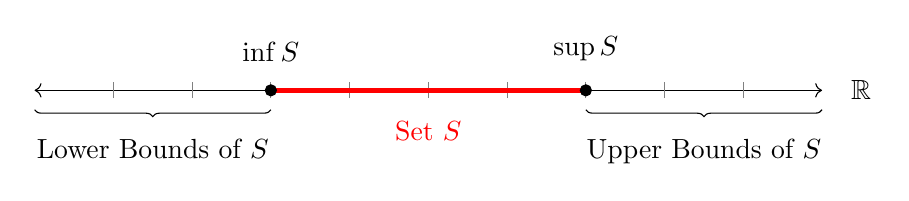
\begin{tikzpicture}
        \coordinate (setstart) at (-2, 0);
        \coordinate (setend) at (2, 0);
        \draw[<->] (-5, 0) -- (5, 0) node[right, xshift=7pt] {$ \mathbb{R} $};
        \draw[decoration={brace, mirror, raise=7pt}, decorate] (-5, 0) --
            (setstart) node[pos=0.5, anchor=north, yshift=-14pt]
            {Lower Bounds of $ S $};
        \draw[decoration={brace, mirror, raise=7pt}, decorate] (setend) --
            (5, 0) node[pos=0.5, anchor=north, yshift=-14pt]
            {Upper Bounds of $ S $};
        \foreach \i in {-4, ..., 4} \draw[gray] (\i, -.1) -- (\i, .1);
        \draw[ultra thick, red] (setstart) -- (setend) node[pos=0.5,
            anchor=north, yshift=-7pt]{Set $ S $};
        \filldraw (setstart) circle (2pt) node[above, yshift=7pt] {$ \inf S $};
        \filldraw (setend) circle (2pt) node[above, yshift=7pt] {$ \sup S $};
    \end{tikzpicture}
    \captionof{figure}{$ S \subset \mathbb{R} $  and its bounding points on the
        real line}
\end{definition}
\begin{definition}{The \texorpdfstring{$ \ell^\infty $}{Ell-Infinity}
        Set of Bounded Sequences}{ell-infinity}
    Consider $ \mathbb{R}^\mathbb{N} $: the set of all sequences of reals. We
    cannot work with this entire space, since many real sequences are unbounded,
    and the $ d_1 $ and $ d_2 $ canonical metrics give rise to non-finite sums.
    Therefore, we consider the set $ \ell^\infty $ as the \emph{set of
    all bounded real sequences}:
    \begin{equation}
        X \in \ell^\infty \iff \exists M > 0 \text{ such that }
            \vert X_n \vert \leq M \text { for all } n \in \mathbb{N}.
    \end{equation}
    Then, the infinity metric is defined in terms of the supremum, since a
    sequence with infinite terms mightn't possess a maximum:
    \begin{equation}
        d_\infty(X, Y) = \sup\left\{\left\vert X_i - Y_i \right\vert \colon
            i \in \mathbb{N}\right\} \text { for } X, Y \in \ell^\infty.
    \end{equation}
\end{definition}
\begin{definition}{The Set of Bounded Functions}{bounded-functions-set}
    $ B([0,1]) $ is the \emph{set of all bounded functions} $ f $ such that
    $ f \colon [0, 1] \to \mathbb{R} $.
\end{definition}
\begin{definition}{The Set of Continuous Functions}{cts-functions-set}
    $ C([0,1]) $ is the \emph{set of all continuous functions} $ f $ such that
    $ f \colon [0, 1] \to \mathbb{R} $.
\end{definition}
\begin{theorem}{The set of bounded functions\texorpdfstring{ over $[0, 1]$}{}
    with the sup-metric forms a metric space}{bounded-is-metric}
    Consider the $ d_\infty $ metric on $ B([0, 1]) $ defined in terms of the
    supremum, such that the upper bound needn't lie in the set:
    \begin{equation}
        d_\infty \colon B([0, 1]) \times B([0, 1]) \to [0, \infty)
            \text{ such that } (f, g) \mapsto \sup\left\{\left\vert f(t) - g(t)
            \right\vert \colon t \in [0, 1] \right\}.
    \end{equation}
    Then, $ \left(B([0, 1]),\, d_\infty\right) $ is a metric space.
    \begin{proof}
        We must verify that $ d_\infty : B([0, 1]) \times B([0, 1]) \to [0,
        \infty) $ satisfies the metric axioms described in
        \cref{definition:metric} for all $ f, g, h \in B([0, 1]) $.
        \begin{itemize}
            \item Since $ f-g $ is a bounded function, there exists an $ M \geq
                0 $ for which $ f(t) - g(t) \leq M $ for all $ t \in [0, 1] $.
                Thus, $ \sup\left\{\left\vert f(t) - g(t) \right\vert \colon t
                \in [0, 1]\right\} \geq 0 $, and $ d_\infty(f, g) \geq 0 $ for
                all $ f, g \in B([0, 1]) $.
            \item \iffforward If $ f = g $, then $ \vert f(t) - g(t) \vert = 0 $
                for all $ t \in [0, 1] $, so $ d_\infty(f, g) = \sup\{0, 0,
                \ldots\} = 0 $.

                \iffbackward Furthermore, if $ d_\infty(f, g) = 0 $, then we
                know that $ \sup\left\{ \left\vert f(t) - g(t) \right\vert
                \colon t \in [0, 1] \right\} = 0 $. We know that $ \vert f(t) -
                g(t) \vert \geq 0 $, so $ \vert f(t) - g(t) \vert = 0 $ follows
                immediately, from which we can conclude that $ f(t) = g(t) $ for
                all $ t \in [0, 1] $, hence $ f = g $.

                Thus, $ d_\infty(f, g) = 0 \iff f = g $.
            \item By the symmetry of the standard metric on $ \mathbb{R} $, the
                symmetry of $ d_\infty $ on $ B([0, 1]) $ follows immediately:
                \begin{align}
                    d_\infty(f, g) &= \sup\left\{ \left\vert f(t) - g(t)
                        \right\vert \colon t \in [0, 1] \right\} \\
                    &= \sup\left\{ \vert g(t) - f(t) \vert \colon t \in [0, 1]
                        \right\} \\
                    &= d_\infty(g, f).
                \end{align}
            \item By the triangularity property of the standard metric on $
                    \mathbb{R} $,
                \begin{align}
                    d_\infty(f, g) &= \sup\left\{ \left\vert f(t) - g(t)
                        \right\vert \colon t \in [0, 1] \right\} \\
                    &= \sup\left\{ \left\vert f(t) - h(t) + h(t) - g(t)
                        \right\vert \colon t \in [0, 1] \right\} \\
                    &\leq \sup\left\{ \left\vert f(t) - h(t) \right\vert \colon
                        t \in [0, 1] \right\} + \sup\left\{ \left\vert h(t) -
                        g(t) \right\vert \colon t \in [0, 1] \right\} \\
                    &= d_\infty(f, h) + d_\infty(h, g),
                \end{align}
                hence $ d_\infty $ possesses the property of triangularity on $
                B([0, 1]) $.
        \end{itemize}
        Thus, $ \left(B([0,1]), d_\infty\right) $ is a metric space.
    \end{proof}
\end{theorem}

\lecture{Norms, Subspaces, and Isometric Maps}
        {Viewer.aspx?id=afbe7e12-8494-4fe3-b73f-b08a009bdc46}{
    Lecture Three opens with a counterexample to challenge a common
    misconception. It continues to introduce the concept of \emph{norms} as
    generalisations of the absolute value function, \emph{metric subspaces}, and
    \emph{isometric maps}, complemented by a simple example.
}{\DTMdisplaydate{2023}{10}{03}{Tuesday}}

\begin{example}{Binary Strings}{binary-strings}
    Despite the examples seen thus far, metric spaces needn't support an
    associated arithmetic or algebraic structure. For instance, let $ \Sigma =
    \{ 0, 1 \}^\mathbb{N} $ be the set of binary strings (sequences of zeroes
    and ones). If $ \sigma = \left(a_n\right)_{n=1}^\infty \in \Sigma $ and $
    \sigma^\prime = \left(b_n\right)_{n=1}^\infty \in \Sigma $, consider the
    distance function $ d \colon \Sigma \times \Sigma \to [0, \infty) $ such
    that
    \begin{equation}
        \left(\sigma, \sigma^\prime\right) \mapsto
        \begin{cases}
            0 &\text{ if } a_n = b_n \quad \forall n \in \mathbb{N}; \\
            1/\min\left\{n \colon a_n \neq b_n\right\} &\text{ otherwise.} \\
        \end{cases}.
    \end{equation}
    Despite there being no inherent algebraic structure or ordering on $ \Sigma
    $, $ d $ is a metric that is inversely proportional with the earliest point
    at which two given binary strings diverge, thus inducing a very natural---
    although unconventional---notion of \emph{distance}.
    \tcblower
    This example was adapted from Ben Green's University of Oxford
    \href{https://courses.maths.ox.ac.uk/course/view.php?id=65}{Metric Spaces
    and Complex Analysis} Michaelmas 2021 course notes.
\end{example}
\begin{definition}{Norm}{norm}
    A \emph{norm} is an abstraction of the absolute value. Suppose that $ V $ is
    a normable vector space. Then $ \vert\vert\cdot\vert\vert \colon V \to
    \mathbb{R} $ is such that, for all $ \vec{x}, \vec{y} \in V $,
    \setaxiomprefix{N}
    \begin{axioms}
        \item $ \vert\vert \vec{x} \vert\vert \geq 0 $;
        \item $ \vert\vert \vec{x} \vert\vert = 0 \iff \vec{x} = \vec{0} $;
        \item $ \vert\vert \lambda \vec{x} \vert\vert = \vert \lambda \vert
            \vert\vert \vec{x} \vert\vert $ for all $ \lambda \in \mathbb{R} $;
        \item $ \vert\vert \vec{x} + \vec{y} \vert\vert \leq \vert\vert \vec{x}
            \vert\vert + \vert\vert \vec{y} \vert\vert $.
    \end{axioms}
    $ V $ equipped with $ \vert\vert \cdot \vert\vert $ is a \emph{normed
    space}. Note that any norm can give rise to a metric; such a metric is
    sometimes called the \emph{metric induced by the norm}.
\end{definition}
\begin{definition}{Metric Subspace}{metric-subspace}
    Suppose that $ (X, d) $ and $ (Y, e) $ are metric spaces. We say that $ X $
    is a \emph{metric subspace} of $ Y $ if $ X \subseteq Y $ and $ d $ is a
    restriction of $ e $ to $ X \times X $.
\end{definition}
\begin{definition}{Isometric Map}{isometric-map}
    Suppose that $ (X, d) $ and $ (Y, e) $ are metric spaces, and that $ \phi
    \colon X \to Y $ is surjective. Then $ \phi $ is called an \emph{isometric
    map} if and only if $ e(\phi(a), \phi(b)) = d(a, b) $ for all $ a, b \in X
    $. This will later be used to define the most rigid definition of
    ``sameness'' for metric spaces.
\end{definition}
\begin{example}{Complex Isometry}{complex-isometry}
    Each $ (a, b) \in \mathbb{R} $ is associated with a unique $ z = a +
    \mathrm{i}b \in \mathbb{C} $ such that $ \Re(z) = a $ and $ \Im(z) = b $.
    Notice that $ (a, b) \mapsto a + \mathrm{i}b $ is a bijective map from $
    \mathbb{R}^2 $ to $ \mathbb{C} $, and hence qualifies as an isometry.
\end{example}

\lecture{Introduction to the Topology of Metric Spaces}
        {Viewer.aspx?id=3a47174e-ed9d-413d-b309-b08c009bdb8e}{
    Lecture Four begins an investigation into the topology of a metric space. In
    particular, we introduce \emph{open and closed balls}, \emph{interior
    points}, \emph{boundary points}, and \emph{exterior points}, and define
    \emph{open} and \emph{closed} sets in terms of these concepts. We take an
    example metric space and rigorously compute its interior, boundary, and
    exterior, and finally show (by example) that considering objects as either
    subsets or subspaces can vastly alter their topological properties.
}{\DTMdisplaydate{2023}{10}{05}{Thursday}}

\begin{definition}{Open and Closed Balls}{balls}
    Suppose that $ (X, d) $ is a metric space, and that $ x_0 \in X $. For every
    $ \epsilon > 0 $, we define the \emph{open ball centered at $ x_0 $ with
    radius $ \epsilon $} to be the set $ B(x_0, \epsilon) = \left\{ x \in X
    \colon d(x, x_0) < \epsilon \right\} $. Analogously, the \emph{closed ball
    centered at $ x_0 $ with radius $ \epsilon $} is defined to be the set
    $ \overline{B}(x_0, \epsilon) = \left\{ x \in X \colon d(x, x_0) \leq
    \epsilon \right\} $.

    \centering
    \begin{minipage}{.5\linewidth}
        \centering
        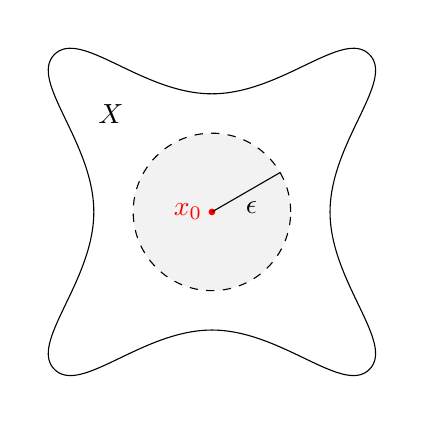
\begin{tikzpicture}
            \pic at (0, 0) {squarespace};
            \draw[fill=ballfill, dashed] (0, 0) circle[radius=1] node[above
                left=1cm]{$ X $};
            \filldraw[red] (0, 0) circle (1pt) node[left] {$ x_0 $};
            \draw (0, 0) -- ++(30:1cm) node[anchor=north, pos=0.5, xshift=2pt]
                {$ \epsilon $};
        \end{tikzpicture}
        \captionof{figure}{The open ball $ B(x_0, \epsilon) \subset X $}
    \end{minipage}\hfill
    \begin{minipage}{.5\linewidth}
        \centering
        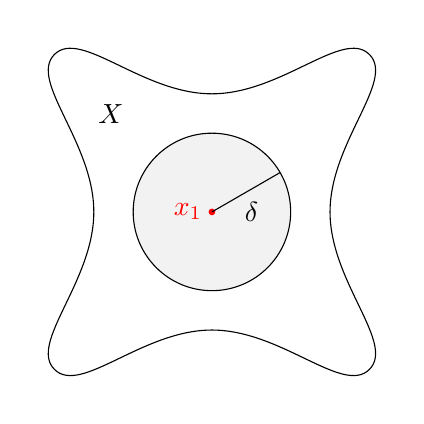
\begin{tikzpicture}
            \pic at (0, 0) {squarespace};
            \draw[fill=ballfill] (0, 0) circle[radius=1] node[above left=1cm]
                {$ X $};
            \filldraw[red] (0, 0) circle (1pt) node[left] {$ x_1 $};
            \draw (0, 0) -- ++(30:1cm) node[anchor=north, pos=0.5, xshift=2pt]
                {$ \delta $};
        \end{tikzpicture}
        \captionof{figure}{The closed ball $ \overline{B}(x_1, \delta)
            \subset X $}
    \end{minipage}
\end{definition}
\begin{definition}{Interior Points}{interior-points}
    Let $ A \subset X $. An \emph{interior point} $ y \in X $ of $ A $ is an
    element for which $ B(y, \epsilon) \subset A $ for some $ \epsilon > 0 $.
    That is, there is an open ball centred at $ y $ with radius $ \epsilon $
    that is completely contained within $ A $. The set of all such points is
    denoted as $ A^o $, and is called \emph{the interior of $ A $}.
\end{definition}
\begin{definition}{Boundary Points}{boundary-points}
    The element $ y \in X $ is a \emph{boundary point} of $ A $ if and only if
    for any $ \epsilon > 0 $, $ B(y, \epsilon) \cap A \neq \emptyset $ and
    $ B(y, \epsilon) \cap A^c \neq \emptyset $. That is, any open ball centred
    at $ y $ always intersects with $ A $ and its complement $ A^c $. The set of
    all such points is denoted as $ \partial A $, and is called \emph{the
    boundary of $ A $}.
\end{definition}
\begin{definition}{Exterior Points}{exterior-points}
    The element $ y \in X $ is an \emph{exterior point} of A if and only if for
    some $ \epsilon > 0 $, $ B(y, \epsilon) \subset A^c $. That is, there exists
    an open ball centred at $ y $ which intersects only with the complement of
    $ A $; this can also be interpreted as an interior point of the complement.
    The set of all such points is denoted as $ A^e $, and is called \emph{the
    exterior of A}.
\end{definition}
\begin{example}{Illustration of Interior, Boundary, and Exterior Points}
        {int-bound-ext-graphic}
    Consider an ambient space $ X $, and the shaded subset $ A \subseteq X $.
    We can illustrate examples of points from the interior, boundary, and
    exterior of $ A $.

    \begin{minipage}{.3\linewidth}
        \centering
        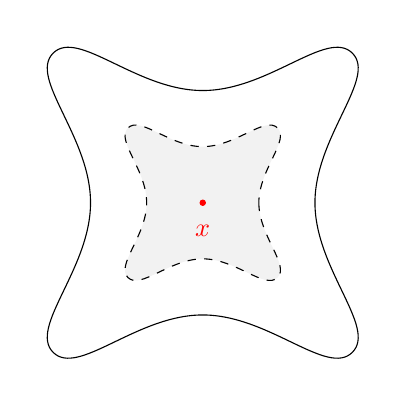
\begin{tikzpicture}[scale=0.95]
            \pic at (0, 0) {squarespace};
            \pic[scale=0.5, every path/.style={fill=ballfill, dashed}] at (0, 0)
                {squarespace};
            \filldraw[red] (0, 0) circle (1pt) node[below, yshift=-5pt] {$ x $};
        \end{tikzpicture}
        \captionof{figure}{An interior point $ x \in A^o $}
    \end{minipage}\hfill
    \begin{minipage}{.3\linewidth}
        \centering
        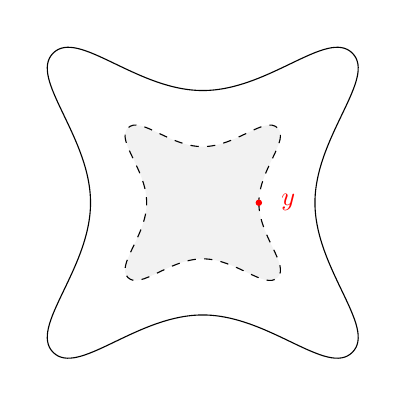
\begin{tikzpicture}[scale=0.95]
            \pic at (0, 0) {squarespace};
            \pic[scale=0.5, every path/.style={fill=ballfill, dashed}] at (0, 0)
                {squarespace};
            \filldraw[red] (.75, 0) circle (1pt) node[right, xshift=5pt]
                {$ y $};
        \end{tikzpicture}
        \captionof{figure}{A boundary point $ y \in \partial A $}
    \end{minipage}\hfill
    \begin{minipage}{.3\linewidth}
        \centering
        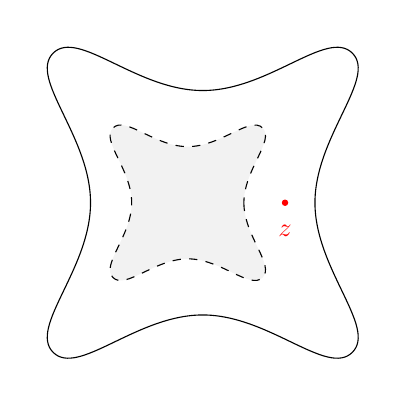
\begin{tikzpicture}[scale=0.95]
            \pic at (.2, 0) {squarespace};
            \pic[scale=0.5, every path/.style={fill=ballfill, dashed}] at (0, 0)
                {squarespace};
            \filldraw[red] (1.3, 0) circle (1pt) node[below, yshift=-5pt]
                {$ z $};
        \end{tikzpicture}
        \captionof{figure}{An exterior point $ z \in A^e $}
    \end{minipage}

    Note that the interior, boundary, and exterior are mutually disjoint and can
    be placed under the disjoint union operation to form the entire ambient
    space. This fact is henceforth denoted by ``$ A^o \coprod \partial A \coprod
    A^e = X $'' for $ A \subseteq X $.
\end{example}
\begin{example}{Finding the interior, boundary, and exterior of a
        set}{int-bound-ext}
    Consider $ (\mathbb{R}, d) $ with $ A = (0, 1] \subset \mathbb{R} $.
    Intuitively, we can conjecture that $ A^o = (0, 1) $, $ \partial A = \{0,
    1\} $, and $ A^e = \mathbb{R} \setminus (0, 1) = (-\infty, 0) \cup (1,
    \infty) $, however these claims must be proven rigorously by (a) showing
    that the conjectured points do belong to the relevant set, and (b) showing
    that the conjectured points are the only elements to belong to the relevant
    set.
    \begin{itemize}
        \item First consider the interior. Take $ x \in (0, 1) $. By
            \cref{definition:interior-points}, we want to show that there is an
            $ \epsilon > 0 $ such that $ B(x, \epsilon) \subset (0, 1] = A $.
            Set $ \epsilon_1 \coloneq x $, and $ \epsilon_2 \coloneq 1-x $.
            Given that $ 0 < x < 1 $, we can take an $ \epsilon \coloneq
            \min\{ \epsilon_1, \epsilon_2 \} $. Then, since $ \epsilon/2 <
            \epsilon_1, \epsilon_2 $,
            \begin{equation}
                B(x, \epsilon/2) = \left\{ y \in \mathbb{R} \colon d(x, y) <
                    \epsilon/2 \right\} \subset A.
            \end{equation}
            This proves that $ (0, 1) \subseteq A^o $.

            We now need to eliminate the remaining candidates in $ \mathbb{R}
            \setminus (0, 1) $ from having possible membership in $ A^o $. The
            points $ x < 0 $ and $ x > 1 $ can be discarded immediately, since
            any open ball centred at these points could never lie totally within
            $ A $, due to their positive radii $ \epsilon $. Finally, we need to
            show that $ \{0,1\} \not\subset A^o $. Without loss of generality,
            pick $ x = 1 $, and take an $ \epsilon > 0 $ to consider the open
            ball $ B(x, \epsilon) $. Any such ball would contain a point that is
            strictly greater than 1, and hence would contain points outside of $
            A $. Thus, $ x \not\in A^o $, and $ A^o = (0, 1) $ as claimed.
        \item Now consider the boundary, as described in
            \cref{definition:boundary-points}. We claim that $ \{0, 1\} =
            \partial A $, and first demonstrate that $ \{0, 1\} \subseteq
            \partial A $.  Without loss of generality, we show that $ 0 \in
            \partial A $. Let $ \epsilon > 0 $, and consider $ B(0, \epsilon) =
            (-\epsilon, \epsilon) $. Clearly, since $ \epsilon > 0 $, $
            (-\epsilon, \epsilon) \cap A \neq \emptyset $ and $ (-\epsilon,
            \epsilon) \cap A^c \neq \emptyset $; thus, $ 0 $ is a boundary
            point.

            Now, we show that there are no other boundary points of $ A $ in $
            \mathbb{R} $. We know that $ \mathbb{R} = A^o \coprod \partial A
            \coprod A^e $, hence $ A^o \cup \partial A = \emptyset $, thus $ (0,
            1) \not\subset \partial A $. Without loss of generality for $ x < 0
            $, consider points $ x > 1 $. Therefore, there exists an $ \epsilon
            > 0 $ such that $ x = 1 + \epsilon $. Considering $ B(x, \epsilon/2)
            $, we can see that $ B(x, \epsilon/2) \subset A^c $, which implies
            that $ B(x, \epsilon/2) \cap A = \emptyset $. Thus, $ \{ 0, 1 \} =
            \partial A $.
        \item Finally, consider the exterior, as described in
            \cref{definition:exterior-points}. Recall that the entire space can
            be expressed as a disjoint union, e.g. $ \mathbb{R} = A^o \coprod
            A^e \coprod \partial A $. Hence,
            \begin{align}
                A^e &= \mathbb{R} \setminus \left( A^o \cup \partial A
                    \right) \\
                &= \mathbb{R} \setminus [0, 1] \\
                &= (-\infty, 0) \cup (1, \infty),
            \end{align}
            as conjectured.
    \end{itemize}
\end{example}
\begin{definition}{Open, Closed, and Clopen Sets}{open-closed-clopen-sets}
    Let $ (X, d) $ be a metric space. A subset $ A $ of $ X $ is \emph{open} if
    and only if $ A \cap \partial A = \emptyset $. A subset $ F $ of $ X $ is
    \emph{closed} if and only if $ \partial F \subseteq F $. Note that a set can
    be both open and closed: typical examples are the empty set and the entire
    space; these sets are called \emph{clopen}.

    \centering
    \begin{minipage}{.5\linewidth}
        \centering
        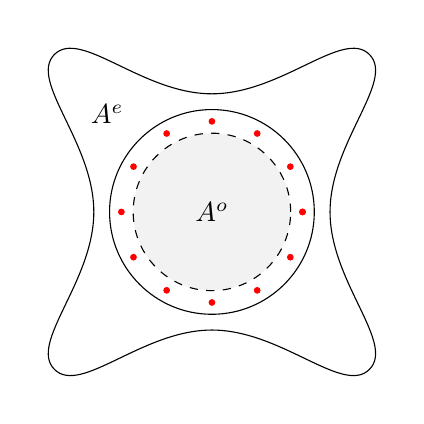
\begin{tikzpicture}
            \pic at (0, 0) {squarespace};
            \draw[fill=ballfill, dashed] (0, 0) circle[radius=1];
            \draw (0, 0) circle[radius=1.3] node {$ A^o $} node[above left=1cm]
                {$ A^e $};
            \foreach \angle in {0, 30, ..., 360}
                \filldraw[red] (\angle:1.15cm) circle (1pt);
        \end{tikzpicture}
        \captionof{figure}{An open set $ A $ does not contain its boundary
            points.}
    \end{minipage}\hfill
    \begin{minipage}{.5\linewidth}
        \centering
        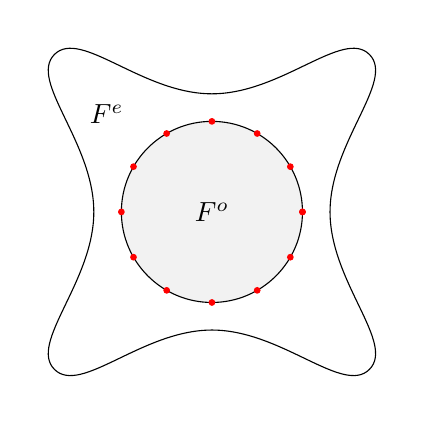
\begin{tikzpicture}
            \pic at (0, 0) {squarespace};
            \draw[fill=ballfill] (0, 0) circle[radius=1.15] node {$ F^o $}
                node[above left=1cm] {$ F^e $};
            \foreach \angle in {0, 30, ..., 360}
                \filldraw[red] (\angle:1.15cm) circle (1pt);
        \end{tikzpicture}
        \captionof{figure}{A closed set $ F $ contains its boundary points.}
    \end{minipage}
\end{definition}
\begin{example}{Subset vs. Subspace}{subset-subspace}
    Consider $ (\mathbb{R}, d) $ with $ A = (0, 1) \cup (1, 2) $. If $ A $ is
    considered as a \emph{subset} if $ \mathbb{R} $, then $ \partial A = \{0, 1,
    2 \} $. Hence, $ A \cap \partial A = \emptyset $, and $ A $ is open by
    \cref{definition:open-closed-clopen-sets}.  Further, $ A $ is not closed,
    since $ \partial A \not\subseteq A $.

    If $ A $ is considered as a \emph{subspace} of $ \mathbb{R} $, then $
    \partial A = \emptyset $, since $ \{ 0, 1, 2 \} \not\subseteq A $, and we
    cannot consider the points outside of the subspace when determining its
    topology. Hence, $ A $ is closed. But $ A \cap \partial A = \emptyset $,
    since $ \partial A = \emptyset $; thus $ A $ is also open, and is ultimately
    clopen when interpreted as a subspace.
\end{example}

\lecture{Results on the Topology of Metric Spaces}
        {Viewer.aspx?id=dbcb156d-d828-454f-929d-b091009bf65b}{
    Lecture Five proves multiple important theorems: a set is open if and only
    if its complement is closed; a set is open if and only if we can place an
    open ball around every point and stay inside of the set; and an open set can
    be expressed as a union of open balls. We also introduce the notion of
    \emph{a topology} $ T_d $ as the collection of all open subsets, and prove
    theorems related to closure under the familiar union and intersection set
    operations.
}{\DTMdisplaydate{2023}{10}{10}{Tuesday}}\label{sec:topology-results}

\begin{theorem}{A subset is open if and only if its complement is
        closed}{open-subset-closed-complement}
    Consider a set $ A \subseteq X $. Then, $ A $ is open if and only if $ A^c $
    is closed.
    \begin{proof}
        This can be proven by unravelling the definitions of open and closed
        sets (\cref{definition:open-closed-clopen-sets}) and boundary points
        (\cref{definition:boundary-points}).

        \iffforward First, suppose that $ A $ is open.  If $ A = \emptyset $,
        then $ A^c = X $. The entire space is known to be clopen, and thus
        closed. If $ A \neq \emptyset $, then $ A \cap \partial A = \emptyset $,
        and $ \partial A \subseteq A^c $.  We can now see a useful equality by
        using the fact that $ \left(A^c\right)^c = A $:
        \begin{align}
            \partial \left(A^c\right) &= \left\{ y \in X \colon \forall \epsilon
                > 0 \, B(y, \epsilon) \cap A^c \neq \emptyset \land B(x,
                \epsilon) \cap \left(A^c\right)^c \neq \emptyset \right\}%
                \label{eqn:boundary-complement-boundary-first}\\
            &= \left\{ y \in X \colon \forall \epsilon > 0 \, B(y, \epsilon)
                \cap A^c \neq \emptyset \land B(x, \epsilon) \cap A \neq
                \emptyset \right\} \\
            &= \partial A.\label{eqn:boundary-complement-boundary-last}
        \end{align}
        Since $ \partial A \subseteq A^c $, and $ \partial A = \partial
        \left(A^c\right) $, we know that $ \partial \left(A^c\right) \subseteq
        A^c $. Hence, $ A^c $ is closed.

        \iffbackward Next, assume that $ A^c $ is closed, hence $ \partial
        \left(A^c\right) \subseteq A^c $. Given that $ \partial A = \partial
        \left(A^c\right) $, $ \partial A \subseteq A^c $. Since $ A^c \cap A =
        \emptyset $, we know that $ \partial A \cap A = \emptyset $, and thus $
        A $ is open.
    \end{proof}
\end{theorem}
\begin{definition}{The topology of a metric space}{topology}
    The \emph{topology} of a metric space $ (X, d) $ is denoted as $ T_d $, and
    is defined to be \emph{the collection of all open subsets of $ X $}. Note
    that since $ T_d \subseteq \mathcal{P}(X) $, for any set $ X $, $ \emptyset,
    X \in T_d $, so $ T_d \neq \emptyset $.
\end{definition}
\begin{theorem}{Equivalence between openness and the existence of open balls}
        {openness-open-balls}
    Let $ A \subseteq X $ be open. Then, every point of $ A $ is an interior
    point of A. Equivalently, $ A $ is open if and only if there is an open ball
    around every point in $ A $ that resides within $ A $:
    \begin{equation}
        \forall x \in A\, \exists \epsilon > 0 \text{ such that } B (x,
        \epsilon) \subseteq A.
    \end{equation}

    \begin{minipage}{\dimexpr.6\linewidth-2em}
        \begin{proof}
            \iffforward First assume that $ A $ is open. By definition, $ A \cap
            \partial A = \emptyset $. If $ A = \emptyset $, then there exists no
            points to select, and the universal quantifier cannot select any
            points for $ x $. If $ A \neq \emptyset $, then there must be at
            least one $ \epsilon > 0 $ such that $ B(x, \epsilon) \subseteq A $
            or $ B(x, \epsilon) \subseteq A^c $ for any $ x \in A $. But, since
            $ x \in A $, it is not possible that $ B(x, \epsilon) $ is entirely
            contained within $ A^c $, since $ x \in B(x, \epsilon) $. Hence, $
            B(x, \epsilon) \subseteq A^c $, as required.

            \iffbackward Next, suppose that $ \forall x \in A\, \exists \epsilon
            > 0 $ such that $ B (x, \epsilon) \subseteq A $. Take any $ x \in A
            $.  Immediately, we can see that $ x \not\in \partial A $, since $
            B(x, \epsilon) \cap A^c = \emptyset $, because $ B(x, \epsilon)
            \subseteq A $. Hence, $ A $ is open.
        \end{proof}
    \end{minipage}\hfill
    \begin{minipage}{.4\linewidth}
        \centering
        \begin{tikzpicture}
            \coordinate (x1point) at (1, 1);
            \coordinate (x2point) at (-1, 1);
            \coordinate (x3point) at (0, -1);
            \draw[dashed] (0, 0) circle (2.7cm);
            \foreach \pt in {1, 2, 3}{
                \filldraw[red] (x\pt point) circle (1pt);
                \draw[dashed, red] (x\pt point) circle (.4cm*\pt+.05cm)
                    node[below] {$ x_\pt $};
                \draw[red] (x\pt point) -- ++(45*\pt:.4cm*\pt+.05cm);
            }
        \end{tikzpicture}
        \captionof{figure}{Every point supports an open ball}
    \end{minipage}
\end{theorem}
\begin{theorem}{The open ball is open}{open-ball-open}
    For any $ x \in X $ and any $ \epsilon > 0 $, $ B(x, \epsilon) \in T_d $.
    Since $ T_d $ is defined to be a collection of open sets, this statement is
    equivalent to the claim that ``\emph{the open ball is open}''.
    \begin{proof}
        Take an $ x \in X $ and construct the open ball $ B(x, \epsilon) $, for
        a fixed $ \epsilon > 0 $. Take $ y \in B(x, \epsilon) $ and let $ \Delta
        \coloneq d(x, y) $. If $ x=y $, then $ B(x, \epsilon) = B(y, \epsilon)
        \subseteq B(x, \epsilon) $, there is nothing to do; therefore, we assume
        that $ x \neq y $, thus $ \Delta > 0 $ and $ 0 < \Delta < \epsilon $.
        Let $ \epsilon^\prime \coloneq \min\left\{ \Delta, \epsilon-\Delta
        \right\} $ and consider $ B(y, \epsilon^\prime/2) $.

        \begin{minipage}{.45\linewidth}
            To show the openness of the open ball, it is sufficient to show that
            $ B(y, \epsilon^\prime/2) \subseteq B(x, \epsilon) $. By the
            triangle inequality on $ d $, for any $ z \in B(y,
            \epsilon^\prime/2) $,
            \begin{align}
                d(x, z) &\leq d(x, y) + d(y, z) \\
                &\leq \Delta + \epsilon^\prime/2 \\
                &= \Delta + \min\left\{\Delta, \epsilon-\Delta\right\}/2 \\
                &\leq \Delta + (\epsilon-\Delta)/2 \\
                &< \Delta + \epsilon - \Delta \\
                &= \epsilon
            \end{align}
        \end{minipage}\hfill
        \begin{minipage}{.5\linewidth}
            \centering
            \begin{tikzpicture}
                \coordinate (xpoint) at (0, 0);
                \coordinate (ypoint) at (0, 1.5);
                \draw[dashed] (xpoint) circle (2.7cm);
                \draw (xpoint) -- ++(-30:2.7cm) node[anchor=south, pos=0.5,
                    xshift=3pt, yshift=3pt] {$ \epsilon $};
                \filldraw[blue] (xpoint) circle (1pt) node[left, xshift=-3pt]
                    {$ x $};
                \filldraw[red] (ypoint) circle (1pt) node[right, xshift=3pt]
                    {$ y $};
                \draw[blue, dotted] (xpoint) -- (ypoint);
                \draw[dashed, red] (ypoint) circle (1cm);
                \draw[red] (ypoint) -- ++(120:1cm) node[left, pos=.5,
                    yshift=-3pt] {$ \frac{\epsilon^\prime}{2} $};
                \node[blue] at (-.75, -1.3)
                    {$ \left[\,\Delta = d(x, y)\,\right] $};
            \end{tikzpicture}
            \captionof{figure}{Careful construction of
                $ B(y, \epsilon^\prime/2) $}
        \end{minipage}

        Thus, $ z \in B(x, \epsilon) $ for all $ z \in B(y, \epsilon^\prime/2)
        $. Therefore, $ B(y, \epsilon^\prime/2) \subseteq B(x, \epsilon) $, and
        open balls are indeed open.
    \end{proof}
\end{theorem}
\begin{theorem}{Elements of the topology are unions of open balls}
        {topology-open-balls}
    If $ A \in T_d $ and $ A \neq \emptyset $, then $ A $ is a union of open
    balls.
    \begin{proof}
        Suppose that $ A \neq \emptyset $ and is open. Take any $ x \in A $, and
        we know by \cref{theorem:openness-open-balls} that there exists an $
        \epsilon > 0 $ such that $ B(x, \epsilon) \subseteq A $. Then, we claim
        that
        \begin{equation}
            A = \bigcup_{x \in A} B\left(x, \epsilon(x)\right)
            \underbrace{\iff \left[
                A \subseteq \bigcup_{x \in A} B\left(x, \epsilon(x)\right)
                    \,\land\, A \supseteq \bigcup_{x \in A} B\left(x,
                    \epsilon(x)\right)
                \right]}_{\text{true by the principle of double-inclusion}}.
        \end{equation}
        The leftmost conjunctive on the right-hand-side is clearly true: by
        placing an open ball of strictly positive radius around every point in $
        A $, the entire set will be covered, since $ x \in B(x, \epsilon) $ for
        any $ x $ and $ \epsilon > 0 $. The rightmost conjunctive is also true,
        since each individual ball is wholly contained within $ A $, and taking
        the union of all such interior balls cause any elements to ``escape''
        the set in which they reside. Hence, $ A $ is the union of the open
        balls centered about every point in $ A $.
    \end{proof}
\end{theorem}
\begin{theorem}{Any union of open sets is open}{open-union-open}
    Take \emph{any} (finite, countably infinite, or uncountable) collection of
    open sets $ \Lambda \subseteq T_d $. Then, for any $ \Lambda $,
    \begin{equation}
        \bigcup_{\Omega \in \Lambda} \Omega \in T_d \text { is open.}
    \end{equation}
    \begin{proof}
        Take $ x \in \bigcup_{\Omega \in \Lambda} \Omega $. Thus, there exists
        an open $ \Omega(x) $ such that $ x \in \Omega(x) $. By
        \cref{definition:open-closed-clopen-sets}, there exists an $ \epsilon >
        0 $ such that $ B(x, \epsilon) \subseteq \Omega(x) $. By transitivity,
        $ B(x, \epsilon) \subseteq \bigcup_{\Omega \in \Lambda} \Omega $, and
        every union of open sets is open by \cref{theorem:topology-open-balls}.
    \end{proof}
\end{theorem}
\begin{example}{Non-finite open sets are not closed under intersection}
        {non-finite-intersection-counterexample}
    Take $ (\mathbb{R}, d) $ and consider $ I_n \coloneq \left(-1/n, 1/n\right)
    $. Under infinite intersection, we calculate the singleton:
    \begin{equation}
        \bigcap_{n=1}^\infty I_n = \{0\}.
    \end{equation}
    It is known that all singletons are not open---since any $ B(x, \epsilon) $
    with $ \epsilon > 0 $ would exceed the bounds of $ \{x\} $---despite each
    individual $ I_n $ being open. Thus, the union property shown in
    \cref{theorem:open-union-open} does not apply with such generality to
    intersections.

    \centering
    \begin{tikzpicture}
        \coordinate (linestart) at (-5, 0);
        \coordinate (lineend) at (5, 0);
        \draw[<->] (linestart) -- (lineend) node[right, xshift=7pt]
            {$ \mathbb{R} $}; % Number line
        \foreach \i in {1, ..., 5}{
            \draw (-4/\i, .2) arc[start angle=90, end angle=270, radius=.2];
                % Left arc
            \draw (4/\i, .2) arc[start angle=90, end angle=-90, radius=.2];
                % Right arc
            \draw[<->] (-4/\i, -\i*.5-.5) -- (4/\i, -\i*.5-.5); % Interval
            \node at (5, -\i*.5-.5) {$ I_{\i} $}; % Interval marker
            \draw[dotted] (-4/\i, -\i*.5-.5) -- (-4/\i, .2); % Left dotted line
            \draw[dotted] (4/\i, -\i*.5-.5) -- (4/\i, .2); % Right dotted line
        }
        \draw (0, .2) -- (0, -.2); % Zero marker
        \node at (0, .6) {$ 0 $}; % Zero label
        \node at (-4, .6) {$ -1 $}; % Negative-one marker
        \node at (4, .6) {$ 1 $}; % Positive-one marker
        \node[xshift=-5pt] at (-2, .6) {$ -1/2 $}; % Negative-one-half marker
        \node at (2, .6) {$ 1/2 $}; % Positive-one-half marker
    \end{tikzpicture}
    \captionof{figure}{Nested intersections $ I_1 $ through $ I_5 $}
\end{example}
\begin{theorem}{Any finite intersection of open sets is closed}
        {open-intersection-open}
    Take \emph{any finite} collection of open sets $ \Omega_1, \ldots, \Omega_N
    \in T_d $. Then,
    \begin{equation}
        \bigcap_{i=1}^N \Omega_i \in T_d \text{ is open.}
    \end{equation}
    \begin{proof}
        If $ \bigcap_{i=1}^N \Omega_i = \emptyset $, then there is nothing
        further to show, since $ \emptyset $ is known to be open and thus a
        member of all topologies $ T_d $. We now assume that the intersection is
        non-empty, from which we take an element $ x $. Thus, there exists an $
        \epsilon_i > 0 $ for which $ B(x, \epsilon_i) \subseteq \Omega_i $. Let
        $ \epsilon \coloneq \min\left\{ \epsilon_1, \ldots, \epsilon_N \right\}
        $; then, $ B(x, \epsilon) \subseteq B(x, \epsilon_i) \subseteq \Omega_i
        $ for any choice of $ i = 1, \ldots, N $. Therefore,
        \begin{equation}
            B(x, \epsilon) \in \bigcap_{i=1}^N \Omega_i,
        \end{equation}
        since $ B(x, \epsilon) $ is a member of \emph{every} $ \Omega_i $. Hence
        we can place an open ball with positive radius around any point and stay
        within the intersection; it is therefore open.
    \end{proof}
    \centering
    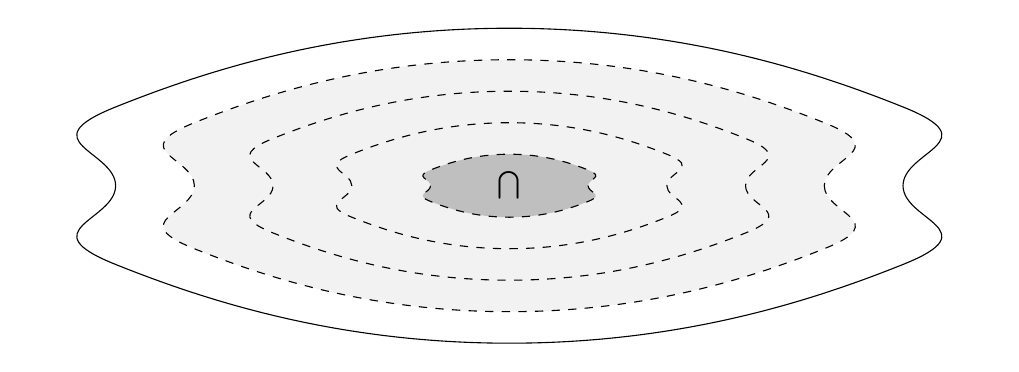
\begin{tikzpicture}
        \pic at (0, 0) {longspace};
        \foreach \i in {.8, .6, .4}{
            \pic[scale=\i, every path/.style={fill=ballfill, dashed}] at (0, 0)
                {longspace};
        }
        \pic[scale=.2, every path/.style={fill=lightgray, dashed}] at (0, 0)
            {longspace} node {$ \bigcap $};
    \end{tikzpicture}
    \captionof{figure}{We consider the intersection of open sets using the
        smallest open ball $ B(x, \epsilon) $.}
\end{theorem}
\begin{theorem}{Summary of \texorpdfstring{$ T_d $}{Open Set} Properties}
        {summary-open-set}
    Let $ (X, d) $ be a metric space, and let $ T_d $ be the topology induced by
    $ d $. Then,
    \setaxiomprefix{T}
    \begin{axioms}
        \item $ \emptyset, X \in T_d $;
        \item For any collection of open sets $ \Lambda \subseteq T_d $,
            $ \bigcup_{\Omega \in \Lambda} \Omega \in T_d $ is open
            (\cref{theorem:open-union-open});\label{axiom:open-union-open}
        \item For any finite collection of open sets $ \Omega_1, \ldots,
            \Omega_N \in T_d $, $ \bigcap_{i=1}^N \Omega_i \in T_d $ is open
            (\cref{theorem:open-intersection-open}).
    \end{axioms}
\end{theorem}

\lecture{Closed Sets \& Topological Equivalence}
        {Viewer.aspx?id=ed63db50-27cd-4d84-8e60-b093009be8af}{
    Lecture Six continues to cover the topology induced by a metric by deriving
    the corresponding properties of closed sets. We introduce the concept of
    \emph{topological equivalence} as weaker method of determining ``sameness''
    between metric spaces. We finally define the \emph{closure} of a set, and
    prove that the closure is closed.
}{\DTMdisplaydate{2023}{10}{12}{Tuesday}}

\begin{theorem}{Summary of Closed Set Properties}{summary-closed-set}
    We can easily derive a dual of \cref{theorem:summary-open-set} for arbitrary
    and finite collections of \emph{closed} sets.
    \setaxiomprefix{F}
    \begin{axioms}
        \item For any collection of closed sets $ \mathcal{F} $,
            \begin{equation}
                \text{For all } F \in \mathcal{F} \text{, } \underbrace{F^c \in
                T_d}_\text{\Cref{theorem:open-subset-closed-complement}}
                \implies\underbrace{\bigcup_{F \in \mathcal{F}} \left( F^c
                \right) \in T_d}_\text{\Cref{axiom:open-union-open}} \implies
                \bigcap_{F \in \mathcal{F}} F \text { is closed,}
            \end{equation}
            since $ \left(\bigcap_{F \in \mathcal{F}} F\right)^c =
            \bigcup_{F \in \mathcal{F}} \left( F^c \right) \in T_d $ by De
            Morgan's laws.
        \item Similarly, for any finite collection of closed sets $ F_1, \ldots,
            F_N $,
            \begin{equation}
                \left( \bigcup_{i=1}^N F_i \right)^c = \bigcap_{i=1}^N F_i^c \in
                T_d \implies \bigcup_{i=1}^N F_i \text{ is closed.}
            \end{equation}
    \end{axioms}
\end{theorem}
\begin{definition}{Topological Equivalence}{topological-equivalence}
    Let $ d $ and $ d^* $ be metrics on a set $ X $. Then, $ (X, d) $ and $ (X,
    d^*) $ are \emph{(topologically) equivalent} if and only if $ T_d = T_{d^*}
    $; that is, $ d $ and $ d^* $ induce the same topologies.
\end{definition}
\begin{theorem}{Determining Topological Equivalence}{determining-top-eq}
    Let $ X $ be a set and let $ d $ and $ d^* $ be metrics on $ X $. Then, $
    T_d = T_{d^*} $ if and only if there exists a scalar $ \lambda > 0 $ for
    which
    \begin{equation}
        \frac{1}{\lambda} d(x, y) \leq d^*(x, y) \leq \lambda d(x, y)
    \end{equation}
    for all $ x, y \in X $.
\end{theorem}
\begin{example}{\texorpdfstring{$ \mathbb{R}^2 $}{The plane} is topologically
        equivalent under the \texorpdfstring{$ d_1 $, $ d_2 $, and $ d_\infty
        $}{standard} metrics}{plane-top-eq}
    Recall the unit circles $ S_1^2 $ (\cref{fig:d1-unit-circle}), $ S_2^2 $
    (\cref{fig:d2-unit-circle}), and $ S_\infty^2 $
    (\cref{fig:dinf-unit-circle}) from \cref{example:unit-circles}. We claim
    (and give an information demonstration to show) that $ T_{d_1} = T_{d_2} =
    T_{d_\infty} $; that is, $ d_1 $, $ d_2 $, and $ d_\infty $ are
    topologically equivalent by \cref{definition:topological-equivalence}.

    We first consider the set $ S_1^2 \eqcolon \Omega $ in the space $
    \left(\mathbb{R}^2, d_2\right) $. Take a point $ x_0 \in \Omega $ and
    construct the open ball $ B(x_0, \epsilon/2) \subseteq S_1^2 $; such a ball
    can be created by considering an $ \epsilon \coloneq \min\left\{ \epsilon_1,
    \epsilon_2, \epsilon_3, \epsilon_4 \right\} $, where $ \epsilon_i $ for $ i
    = 1, 2, 3, 4 $ are the perpendicular distances from $ x_0 $ to the boundary
    of $ \Omega $ by the $ d_2 $ metric. Then, $ \Omega \in T_{d_2} $.

    Next, consider $ S_2^2 \eqcolon \Lambda $ in the space $ \left(\mathbb{R}^2,
    d_1\right) $. Constructing open balls in $ d_1 $ around the points in $
    \Lambda $ is easier still, since we only need to consider `diamonds' which
    lie entirely within the Euclidean $ d_2 $ unit circle. By covering the
    entire set, we can conclude that $ \Lambda \in T_{d_1} $.

    Intuitively, we can see that the metrics $ d_1 $ and $ d_2 $ induce the same
    topologies; analogous arguments apply for establishing the equivalences to $
    d_\infty $.

    \centering
    \begin{minipage}{.45\linewidth}
        \centering
        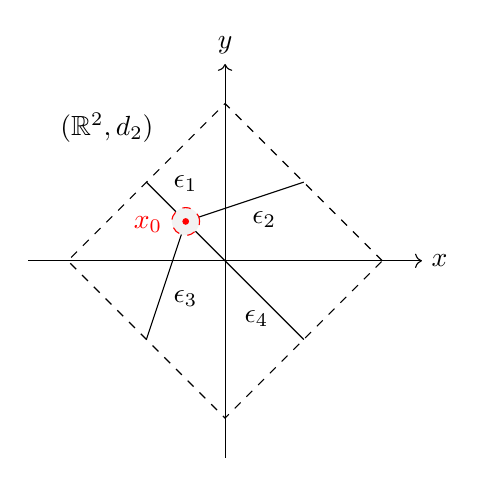
\begin{tikzpicture}
            \coordinate (x0point) at (-.5, .5);
            \draw[->] (-2.5, 0) -- (2.5, 0) node[right] {$x$};
            \draw[->] (0, -2.5) -- (0, 2.5) node[above] {$y$} node[left=1.5cm,
                below=.5cm] {$ (\mathbb{R}^2, d_2) $};
            \node[diamond, dashed, draw, minimum width=4cm, minimum height=4cm]
                {};
            \draw (x0point) -- (-1, 1) node[above, pos=.5, xshift=7pt]
                {$ \epsilon_1 $};
            \draw (x0point) -- (1, 1) node[below, pos=.5, xshift=7pt]
                {$ \epsilon_2 $};
            \draw (x0point) -- (-1, -1) node[below, pos=.5, xshift=7pt]
                {$ \epsilon_3 $};
            \draw (x0point) -- (1, -1) node[below, pos=.6, yshift=-3pt]
                {$ \epsilon_4 $};
            \draw[red, dashed, fill=ballfill] (x0point) circle (5pt);
            \filldraw[red] (x0point) circle (1pt) node[left, red, xshift=-5pt,
                yshift=-1pt] {$ x_0 $};
        \end{tikzpicture}
        \captionof{figure}{Considering the $ d_1 $-defined unit circle $ \Omega
            $ as an open set in the $ \left(\mathbb{R}^2, d_2\right) $ space.}
    \end{minipage}\hfill
    \begin{minipage}{.45\linewidth}
        \centering
        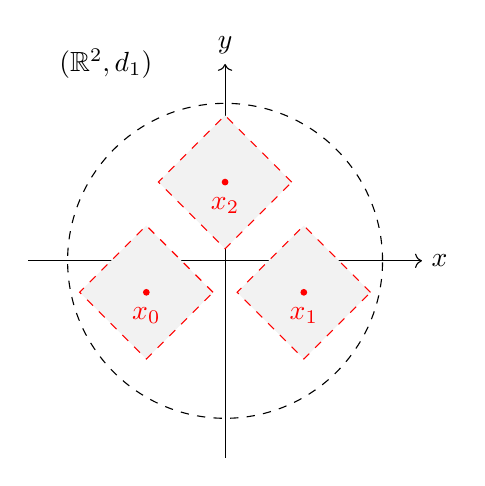
\begin{tikzpicture}
            \coordinate (x0point) at (-1, -.4);
            \coordinate (x1point) at (1, -.4);
            \coordinate (x2point) at (0, 1);
            \draw[->] (-2.5, 0) -- (2.5, 0) node[right] {$x$};
            \draw[->] (0, -2.5) -- (0, 2.5) node[above] {$y$} node[left=.8cm]
                {$ (\mathbb{R}^2, d_1) $};
            \draw[dashed] (0, 0) circle (2cm);
            \foreach \i in {0, 1, 2} {
                \node[diamond, draw, minimum width=1.7cm, minimum height=1.7cm,
                    dashed, red, fill=ballfill] at (x\i point) {};
                \filldraw[red] (x\i point) circle (1pt) node[below, yshift=-2pt]
                    {$ x_\i $};
            }
        \end{tikzpicture}
        \captionof{figure}{Considering the $ d_2 $-defined unit circle $
            \Lambda $ as an open set in the $ \left(\mathbb{R}^2, d_1\right) $
            space.}
    \end{minipage}
\end{example}
\begin{definition}{Closure}{closure}
    Let $ (X, d) $ be a metric space and $ A \subseteq X $. Then the
    \emph{closure} of $ A $, denoted by $ \overline{A} $, is defined to be $
    \overline{A} = A \cup \partial A $.

    \centering
    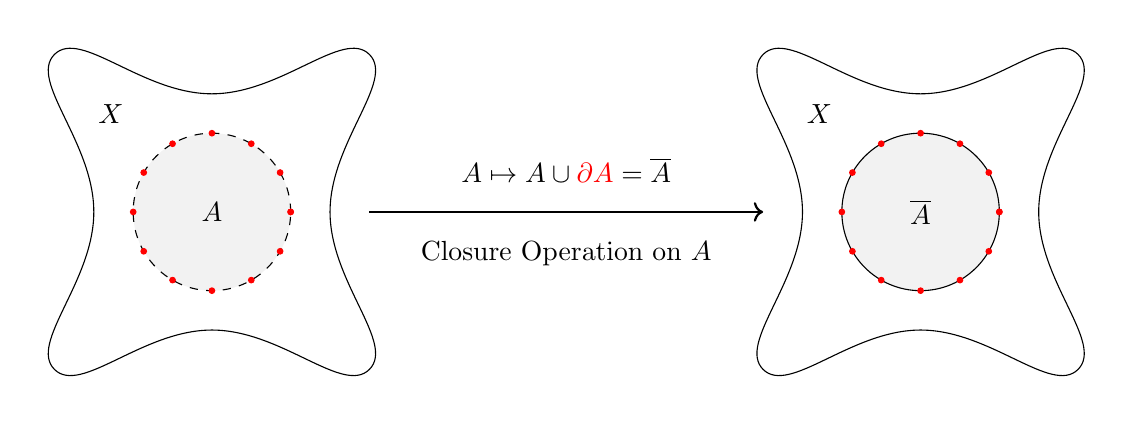
\begin{tikzpicture}
        \coordinate (leftball) at (0, 0);
        \coordinate (rightball) at (9, 0);
        \coordinate (leftbound) at (2, 0);
        \coordinate (rightbound) at (7, 0);
        \pic at (leftball) {squarespace};
        \draw[fill=ballfill, dashed] (leftball) circle[radius=1] node {$ A $}
            node [above left=1cm] {$ X $};
        \pic at (rightball) {squarespace};
        \draw[fill=ballfill] (rightball) circle[radius=1] node
            {$ \overline{A} $} node [above left=1cm] {$ X $};
        \foreach \i in {0, 30, ..., 360} {
            \filldraw[red] (leftball)++(\i:1cm) circle (1pt);
            \filldraw[red] (rightball)++(\i:1cm) circle (1pt);
        }
        \draw[->, thick] (leftbound) -- (rightbound) node [above, pos=.5,
            yshift=7pt] {$ A \mapsto A \cup {\color{red}\partial A} =
            \overline{A} $} node [below, pos=.5, yshift=-7pt]
            {Closure Operation on $ A $};
    \end{tikzpicture}
    \captionof{figure}{Encapsulating the boundary of an open set $ A $ is the
    most `efficient' way of generating a closed set $ \overline{A} $ with the
    same interior $ A^o $.}
\end{definition}
\begin{theorem}{The closure is closed}{closure-closed}
    For an open set $ A \subseteq X $, the closure $ \overline{A} $ is closed.
    \begin{proof}
        By \cref{theorem:open-subset-closed-complement}, $ \overline{A} $ is
        closed if and only if $ \left(\overline{A}\right)^c $ is open. If $
        \left(\overline{A}\right)^c = \emptyset $, then we are done since the
        empty set is known to be open; thus we assume that $
        \left(\overline{A}\right)^c \neq \emptyset $. To prove the openness of
        this non-empty set, we consider an arbitrary point $ x \in
        \left(\overline{A}\right)^c $ and construct an $ \epsilon > 0 $ such
        that $ B(x, \epsilon) \subseteq \left(\overline{A}\right)^c $.

        Since $ \overline{A} = A \cup \partial A $, $ x \not\in A $ and $ x
        \not\in \partial A $. We can use rules from first-order logic combined
        with De Morgan's laws to negate the definition of a boundary point shown
        in \cref{definition:boundary-points}:
        \begin{align}
            x \in \left(\partial A\right)^c &= \left\{ y \in X \colon \forall
                \epsilon > 0 \, B(y, \epsilon) \cap A \neq \emptyset \land B(y,
                \epsilon) \cap A^c \neq \emptyset \right\}^c \\
            &= \left\{ y \in X \colon \forall \epsilon > 0 \, B(y, \epsilon)
                \cap A = \emptyset \lor B(y, \epsilon) \cap A^c = \emptyset
                \right\} \\
            &= \left\{ y \in X \colon \forall \epsilon > 0 \, B(y, \epsilon)
                \subseteq A^c \lor B(y, \epsilon) \subseteq A \right\}
        \end{align}
        Since $ x \not\in A $, $ B(x, \epsilon) \subseteq A^c $ is the only
        possibility. We also require that $ x \not\in \partial A $, so we need
        to show that there is an $ \epsilon > 0 $ such that $ B(x, \epsilon)
        \cap \partial A = \emptyset $. By way of contradiction, suppose that
        there exists a $ y \in B(x, \epsilon) $ such that $ y \in \partial A $.
        By definition \cref{definition:boundary-points}, for all $ \delta > 0 $,
        \begin{equation}
            B(y, \delta) \cap A \neq \emptyset \text{ and } B(y, \delta) \cap
            A^c \neq \emptyset.
        \end{equation}
        If $ d(x, y) \eqcolon \epsilon^* < \epsilon $, and $ \hat{\epsilon}
        \coloneq \min\left\{ \epsilon^*, \epsilon - \epsilon^* \right\} $, then
        $ B(y, \hat{\epsilon}/2) \subseteq B(x, \epsilon) $. But $ B(y,
        \hat{\epsilon}) \cap A \neq \emptyset $. This is a contradiction: no
        such $ y $ can exist, so $ \left(\overline{A}\right)^c $ is open, and $
        \overline{A} $ is closed.
    \end{proof}
    \centering
    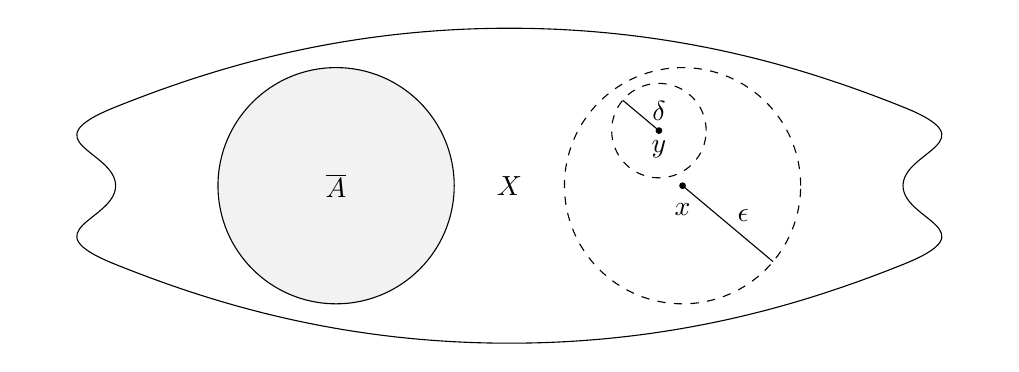
\begin{tikzpicture}
        \coordinate (apos) at (-2.2, 0);
        \coordinate (xpos) at (2.2, 0);
        \coordinate (ypos) at (1.9, .7);
        \pic at (0, 0) {longspace};
        \node at (0, 0) {$ X $};
        \draw[fill=ballfill] (apos) circle (1.5cm) node {$ \overline{A} $};
        \draw[dashed] (xpos) circle (1.5cm);
        \filldraw (xpos) circle (1pt) node[below, yshift=-3pt] {$ x $};
        \draw (xpos) -- ++(320:1.5cm) node[right, pos=.5, yshift=3pt]
            {$ \epsilon $};
        \draw[dashed] (ypos) circle (.6cm);
        \filldraw (ypos) circle (1pt) node[below] {$ y $} node[above]
            {$ \delta $};
        \draw (ypos) -- ++(140:.6cm);
    \end{tikzpicture}
    \captionof{figure}{The open ball $ B(x, \epsilon) $ lies entirely within the
        complement of the closure of $ A $, within which $ B(y, \delta) $ is
        nested.}
\end{theorem}

\lecture{Limit Points and their Consequences}{}{
    Lecture Seven demonstrates that a space is closed if and only if it is equal
    to its own closure, and moves to introduce the topic of
    limit/accumulation/cluster points whilst proving some useful related
    properties.
}{}

\begin{theorem}{Relationships between a closed set and its
        closure}{closed-set-closure}
    If $ A \subseteq X $ is closed, then $ A = \overline{A} $; if $ A =
    \overline{A} $, then $ A $ is closed. That is, $ A $ is closed if and only
    if $ A = \overline{A} $.
    \begin{proof}
        \iffforward If $ A = \overline{A} $, then $ \overline{A} $ is closed by
        \cref{theorem:closure-closed}. Thus $ A $ is closed.

        \iffbackward If $ A $ is closed, then $ \overline{A} = A \cup \partial A
        $ by \cref{definition:closure}. By
        \cref{definition:open-closed-clopen-sets}, $ \overline{A} = \partial A
        \cup \overline{A} = A $.
    \end{proof}
\end{theorem}
\begin{definition}{Limit/Accumulation/Cluster Points}{limit-points}
    \begin{minipage}{.6\linewidth}
        Let $ (X, d) $ be a metric space, and $ A \subseteq X $. A \emph{limit
        point} $ y \in X $ of $ A $ is an element of $ X $ for which
        \begin{equation}
            \left[ B(y, \epsilon) \setminus \{y\} \right] \cap A \neq \emptyset
            \text{ for all } \epsilon > 0.
        \end{equation}
        The \emph{derived set} of $ A $ is denoted $ A^\prime $, and is defined
        to be the set of all limit points of $ A $. Equivalently (in the context
        of metric spaces, but not the more general topological spaces), we can
        say that $ y \in X $ is a limit point of $ A $ if, for any $ \epsilon >
        0 $, the intersection $ B(y, \epsilon) \cap A $ contains infinitely many
        points of $ A $. Limit points are sometimes called \emph{accumulation
        points} or \emph{cluster points}.
    \end{minipage}\hfill
    \begin{minipage}{.35\linewidth}
        \centering
        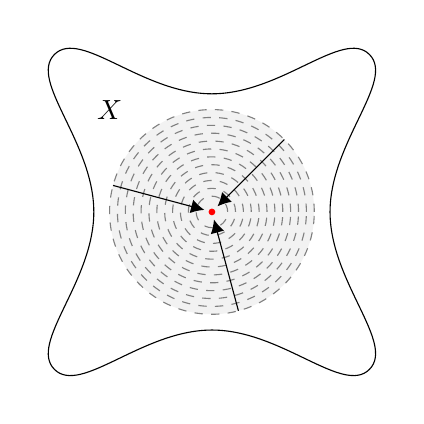
\begin{tikzpicture}
            \pic at (0, 0) {squarespace};
            \node at (-1.3, 1.3) {$ X $};
            \fill[ballfill] (0, 0) circle (1.3cm);
            \foreach \radius in {1.3, 1.2, ..., .1}
                \draw[dashed, gray] (0, 0) circle (\radius cm);
            \filldraw[red] (0, 0) circle (1pt);
            \foreach \angle in {45, 165, 285}
                \draw[-{Latex[width=5pt]}] (\angle:1.3cm) -- (\angle:.1cm);
        \end{tikzpicture}
        \captionof{figure}{As the open balls contract \emph{ad infinitum}, we
            can still find non-centroid points of $ A $.}
    \end{minipage}
\end{definition}
\begin{theorem}{The closure of a set is the union of the base set and its
        derived set}{closure-limit-union}
    For a set $ A \subseteq X $, $ \overline{A} = A \cup A^\prime $.
    \begin{proof}
        If $ A $ is closed, then the result is immediate: $ \overline{A} = A $
        (by \cref{theorem:closed-set-closure}), so $ A^\prime \subseteq A =
        \overline{A} $. Thus, we assume that $ A $ is open. If $ A^\prime =
        \emptyset $, then $ A^\prime \subseteq \overline{A} $, since $ A $ has
        no limit points; therefore, we also assume that $ A $ is non-empty. We
        will show the equality $ \overline{A} = A \cup A^\prime $ for an open
        non-empty set $ A $ through the principle of double-inclusion.

        \iffforward Without loss of generality, suppose that $ y $ is such that
        $ y \in \partial A $ and $ y \not\in A $. For any choice of $ \epsilon >
        0 $, we know that $ B(y, \epsilon) \cap A \neq \emptyset $. Since $ y
        \not\in A $, there exists a $ y^\prime \neq y \in A, B(y, \epsilon) $.
        This is consistent with \cref{definition:limit-points}. Thus, $ y $ is a
        limit point, so $ A^\prime \subseteq \overline{A} $ and $ A \cup
        A^\prime \subseteq \overline{A} $.

        \iffbackward Given that $ A $ is not closed, there exists a $ y \in
        A^\prime $ such that $ y \not\in A $. Take $ \epsilon > 0 $ and note
        that $ B(y, \epsilon) \cap A \neq \emptyset $ and $ B(y, \epsilon) \cap
        A^c \neq \emptyset $. Thus, by \cref{definition:boundary-points}, $ y $
        is a boundary point. We now unravel the definitions:
        \begin{alignat}{2}
            A \text{ is closed} &\iff \partial A \subseteq A
                &&\text{[\Cref{definition:open-closed-clopen-sets}]} \\
            &\iff A^c \text{ is open}
                &&\text{[\Cref{theorem:open-subset-closed-complement}]}%
                \label{eqn:closure-limit-union-open} \\
            &\iff A^c \cap \partial \left( A^c \right) = \emptyset
                &&\text{[\Cref{definition:open-closed-clopen-sets}]} \\
            &\iff A^c \cap \partial A = \emptyset
                &&\text{[\Crefrange{eqn:boundary-complement-boundary-first}%
                    {eqn:boundary-complement-boundary-last}]} \\
            &\iff \forall x \in A^c,\, \exists \epsilon > 0 \text{ s.t. }
                B(x, \epsilon) \subseteq A^c\quad
                &&\text{[\Cref{eqn:closure-limit-union-open}]} \\
            &\iff A = \overline{A} \\
            &\iff A \supseteq A^\prime
        \end{alignat}
        Hence, $ \overline{A} = A \cup \partial A = A \cup A^\prime $ for any
        $ A \subseteq X $.
    \end{proof}
\end{theorem}
\begin{definition}{Topological Interpretation of Closure}{topological-closure}
    Let $ (X, d) $ be a metric space, and $ A \subseteq X $. Then,
    \begin{equation}
        \overline{A} = \bigcap_{F \in \mathcal{F}} F,
    \end{equation}
    where $ \mathcal{F} $ is the collection of all open supersets of $ A $. This
    means that $ \overline{A} $ is the smallest closed superset of $ A $.
\end{definition}
\begin{definition}{Density}{density}
    Let $ (X, d) $ be a metric space and $ A \subseteq X $. Then $ A $ is said
    to be \emph{dense} in $ X $ if and only if $ \overline{A} = X $.
    Alternatively---but equivalently---for any $ x \in X $ and any $ \epsilon >
    0 $, there exists an $ a \in A $ such that $ d(x, a) < \epsilon $.
\end{definition}

\lecture{Sequences and Convergence}
        {Sessions/List.aspx\#folderID="072999e9-f3bc-4486-98af-b0a000d51b97"}{
    Lecture Eight gives the definition of a \emph{sequence} in a metric space,
    and motivates the study of various properties thereof, such as
    \emph{convergence}. Some examples are provided, with familiar concepts from
    Real Analysis being recast into the more abstract setting of metric and
    topological spaces.
}{\DTMdisplaydate{2023}{10}{19}{Thursday}}

\begin{definition}{Sequence}{sequence}
    A \emph{sequence} in a metric space $ (X, d) $ is an element of $
    X^\mathbb{N} $, where any element $ x \in X^\mathbb{N} $ can be written as a
    countable set $ x = \left\{ x_1, \ldots, x_n, \ldots \right\} $, such that
    $ x_i \in X $ for all $ i \in \mathbb{N} $. Such a sequence is denoted
    \begin{equation}
        \left( x_n \right)_{n \in \mathbb{N}} \text{ or }
        \left( x_n \right)_{n=1}^\infty.
    \end{equation}
\end{definition}
\begin{definition}{Convergence of Sequences (by the Metric)}
        {sequence-convergence-metric}
    Let $ \left( x_n \right)_{n \in \mathbb{N}} $ be a sequence in $ (X, d) $.
    Then, $ \left( x_n \right)_{n \in \mathbb{N}} $ \emph{converges} to $ x \in
    X $ if and only if
    \begin{equation}
        \text{For all } \epsilon > 0 \text{, there exists an } N=N(\epsilon)
        \text{ such that } d(x_n, x) < \epsilon \text{ for all } n > N.
    \end{equation}
    If this is the case, we write $ x_n \to x $ (as $ n \to \infty $), and the $
    x $ is \emph{the} (unique) limit of $ \left(x_n\right)_{n \in \mathbb{N}} $.
    If no such $ x $ exists, then $ \left(x_n\right)_{n \in \mathbb{N}} $ is
    \emph{divergent}.

    \centering
    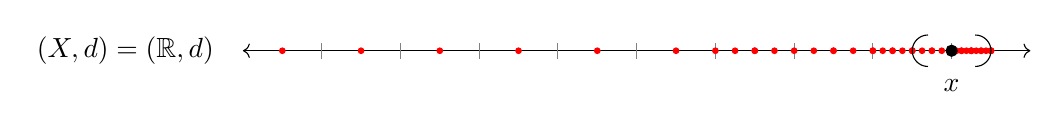
\begin{tikzpicture}
        \draw[<->] (-5, 0) -- (5, 0) node[pos=0, left, xshift=-7pt] {$ (X, d) =
            (\mathbb{R}, d) $}; % Number line and markings
        \foreach \i in {-4, ..., 4} \draw[gray] (\i, -.1) -- (\i, .1);

        \foreach \i in {-4.5, -3.5, ..., 4.5}
            \filldraw[red] (\i, 0) circle (1pt); % Spacing: 1, Start: -4.5

        \foreach \i in {1, 1.25, ..., 4.5}
            \filldraw[red] (\i, 0) circle (1pt); % Spacing: 0.25, Start: 1

        \foreach \i in {3, 3.125, ..., 4.5}
            \filldraw[red] (\i, 0) circle (1pt); % Spacing: 0.125, Start: 3

        \foreach \i in {4, 4.0625, ..., 4.5}
            \filldraw[red] (\i, 0) circle (1pt); % Spacing: 0.0625, Start: 4

        \filldraw (4, 0) circle (2pt) node[below=7pt] {$ x $};

        \draw (3.7, .2) arc[start angle=90, end angle=270, radius=.2]; % L. arc
        \draw (4.3, .2) arc[start angle=90, end angle=-90, radius=.2]; % R. arc
    \end{tikzpicture}
    \captionof{figure}{A sequence in $ (\mathbb{R}, d) $, where $ d $ is the
        standard metric, converging to an $ x \in \mathbb{R} $. The \emph{zone
        of convergence} $ (x-\epsilon, x+\epsilon) $ is denoted with parentheses
        about $ x $.}
\end{definition}
\begin{definition}{Convergence of Sequences (by the Open Balls)}
        {sequence-convergence-balls}
    An equivalent notion of convergence can be expressed in terms of open balls,
    such that the tail of the sequence exists in the open ball centered at the
    limit. Let $ \left( x_n \right)_{n \in \mathbb{N}} $ be a sequence in $ (X,
    d) $. Then, $ \left( x_n \right)_{n \in \mathbb{N}} $ \emph{converges} to $
    x \in X $ if and only if
    \begin{equation}
        \forall \epsilon > 0\, \exists N > 0 \text{ such that } x_n \in B(x,
        \epsilon) \text{ for all } n > N.
    \end{equation}
    That is, for any given $ \epsilon > 0 $, we must find an index $ N $ for the
    sequence $ (x_n)_{n \in \mathbb{N}} $ after which all points $ x_i\,\, (i >
    N) $ exist within the open ball $ B(x, \epsilon) $. If this holds, then the
    sequence $ (x_n) $ converges to the centre of the open ball $ x $.

    \centering
    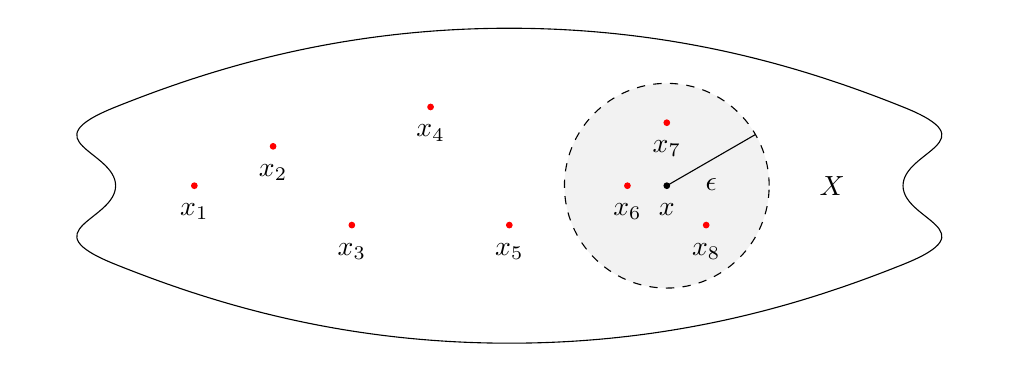
\begin{tikzpicture}
        \coordinate (ballcentre) at (2, 0);
        \pic at (0, 0) {longspace};
        \draw[fill=ballfill, dashed] (ballcentre) circle (1.3cm);
        \filldraw (ballcentre) circle (1pt) node[below, yshift=-3pt] {$ x $};
        \draw (ballcentre) -- ++(30:1.3cm) node[pos=.5, below, yshift=-3pt]
            {$ \epsilon $};
        \node at (4.1, 0) {$ X $};

        \begin{scope}[every path/.style={red}, every node/.style={black, below,
                yshift=-3pt}]
            \filldraw (-4, 0) circle (1pt) node {$ x_1 $};
            \filldraw (-3, .5) circle (1pt) node {$ x_2 $};
            \filldraw (-2, -.5) circle (1pt) node {$ x_3 $};
            \filldraw (-1, 1) circle (1pt) node {$ x_4 $};
            \filldraw (0, -.5) circle (1pt) node {$ x_5 $};
            \filldraw (1.5, 0) circle (1pt) node {$ x_6 $};
            \filldraw (2, .8) circle (1pt) node {$ x_7 $};
            \filldraw (2.5, -.5) circle (1pt) node {$ x_8 $};
        \end{scope}
    \end{tikzpicture}
    \captionof{figure}{A sequence converging within the bounds of an arbitrarily
    sized open ball centred at the limit. In this example, $ N = 5 $, since all
    sequence points $ x_6, x_7, x_8, \ldots $ belong to the pictured open ball.}
\end{definition}
\begin{definition}{Convergence of Sequences (by the convergence of a real
        sequence)}{sequence-convergence-real}
    We can also use results from Real Analysis to consider the real sequence
    generated by the distances between each point in the space and the proposed
    limit $ x $. For a sequence $ \left( x_n \right)_{n \in \mathbb{N}} $ in a
    metric space $ (X, d) $,
    \begin{equation}
        \lim_{n \to \infty} x_n = x \iff \lim_{n \to \infty} d(x_n, x) \to 0.
    \end{equation}
\end{definition}
\begin{theorem}{Convergences of Real-Dimensional Vector
        Spaces}{vector-space-convergence}
    In $ \mathbb{R}^k $ with any $ d_1 $, $ d_2 $, or $ d_\infty $ metrics,
    \emph{overall convergence is equivalent to simultaneous component-wise
    convergence}. That is, for $ \vec{x}_n \in \mathbb{R}^k $ with $ n \in
    \mathbb{N} $,
    \begin{equation}
        \lim_{n \to \infty} \vec{x}_n \to \vec{x} \iff
        \lim_{n \to \infty} x_i^{(n)} \to x_i \text{ for each } i \in \left\{1,
        \ldots, k \right\}.
    \end{equation}
    Note that $ \vec{x} = (x_1, \ldots, x_k) $ denotes a general
    vector/candidate limit, and $ \vec{x}_n = \left(x_1^{(n)}, \ldots,
    x_k^{(n)}\right) $ denotes a $ k $-dimensional vector in the sequence at
    index $ n $. For this demonstration, we will consider the specific case of
    $ \left(\mathbb{R}^k, d_\infty\right) $.
    \begin{proof}
        \iffforward Suppose that $ \vec{x}_n \to \vec{x} $ as $ n \to \infty $.
        We want to show that, for each $ i \in \left\{ 1, \ldots, k \right\} $,
        the components converge such that $ x_i^{(n)} \to x_i $ as $ n \to
        \infty $. Let $ \epsilon > 0 $ be given. Since $ \lim_{n \to \infty}
        \vec{x}_n = \vec{x} $, there exists an $ N(\epsilon) > 0 $ such that
        $ d_\infty(\vec{x}_n, \vec{x}) < \epsilon $ for all $ n > N $. By
        recalling the mapping definition of $ d_\infty $ from
        \cref{definition:canon-metrics}, we can derive that
        \begin{equation}
            \max_{1 \leq i \leq k} \left\vert x_i^{(n)} - x_i \right\vert <
            \epsilon \text{ for all } n > N.
        \end{equation}
        By the nature of the maximum function, we can generalise this inequality
        to all choices of $ i \in \left\{ 1, \ldots, k \right\} $:
        \begin{equation}
            \left\vert x_i^{(n)} - x_i \right\vert < \epsilon \text{ for all } n
            > N \text{ for all } i \in \left\{1, \ldots, k \right\}.
        \end{equation}
        We can immediately arrive at the desired limit for the real sequence: $
        \lim_{n \to \infty} x_i^{(n)} = x_i $ for all $ i \in \left\{ 1, \ldots,
        k \right\} $.

        \iffbackward Now suppose that $ \lim_{n \to \infty} x_i^{(n)} = x_i $
        for all $ i \in \left\{ 1, \ldots, k \right\} $, and let $ \epsilon > 0
        $ be given. Then, for any suitable choice of $ i $, there exists an $
        N_i(\epsilon) > 0 $ such that $ \left\vert x_i^{(n)} - x_i \right\vert <
        \epsilon $ for all $ n > N_i $.
        \begin{equation*}
            \renewcommand\arraystretch{1.5}
            \begin{matrix}
                \vec{x}_1 & \vline & x_1^{(1)} & x_2^{(1)} & x_3^{(1)} & \ldots
                    & x_k^{(1)} \\
                \vec{x}_2 & \vline & x_1^{(2)} & x_2^{(2)} & x_3^{(2)} & \ldots
                    & x_k^{(2)} \\
                \vec{x}_3 & \vline & x_1^{(3)} & x_2^{(3)} & x_3^{(3)} & \ldots
                    & x_k^{(3)} \\
                \vdots & \vline & \vdots & \vdots & \vdots & \ddots & \vdots \\
                \vdots & \vline & \multirow{2}{*}{$ \begin{cases}
                    ~~\color{red}{N_1} \\ ~~~\vdots \end{cases} $} &
                    \big\downarrow & \color{red}{N_3} &
                    \big\downarrow & \color{red}{N_k} &
                    \multirow{2}{*}{\hspace{-1ex} $ \begin{rcases}
                    \vphantom{~}\\\vphantom{~}\end{rcases} $}
                    \\ % What the fuck?
                \vdots & \vline & & \color{red}{N_2} & \vdots & \color{red}{N_j}
                & \vdots \\ & & \multicolumn{6}{c}{\text{Zones of Convergence}}
            \end{matrix}
        \end{equation*}
        Take $ N \coloneq \max\left\{ N_1, \ldots, N_k \right\} $, such that $ N
        $ is a sufficiently large index to induce convergence on all component
        sequences. That is,
        \begin{equation}
            \max_{1 \leq i \leq k} \left\vert x_i^{(n)} - x_i \right\vert <
            \epsilon \text{ for all } n > N.
        \end{equation}
        Thus, $ \lim_{n \to \infty} x_i^{n} = x_i $ for all $ i \in \left\{ 1,
        \ldots, k \right\} $, as desired.
    \end{proof}
\end{theorem}
\begin{example}{Convergence of Continuous Functions}{function-convergence}
    Consider the sequence $ \left( f_n \right)_{n=1}^\infty $ where $ f_n
    \in C\left( [0, 1] \right) $ and $ t \mapsto t^n $. We claim the
    following:

    \begin{enumerate}
        \item In $ d_2 $, $ \left(f_n\right)_{n=1}^\infty $ converges to
            zero;
        \item In $ d_\infty $, $ \left(f_n\right)_{n=1}^\infty $ diverges.
    \end{enumerate}
    First consider the sequence under the $ d_2 $ metric. In general, we
    know that $ x_n \to x $ as $ n \to \infty $ if and only if $ d(x_n, x)
    \to 0 $ as $ n \to \infty $. Therefore, we compute $ d_2(f_n, 0) $:
    \begin{align}
        d_2(f_n, 0) &= \left[ \int_0^1 \left\vert f_n(t) \right\vert^2 \,
            \mathrm{d}t \right]^{1/2} \\
        &= \sqrt{\frac{1}{2n+1}}
    \end{align}

    Given that $ \lim_{n \to \infty}\sqrt{1/(2n+1)} = 0 $, we can conclude that
    $ f_n \to 0 $ as $ n \to \infty $. Next considering the sequence under the
    $ d_\infty $ metric, recall that, for all $ n \in \mathbb{N} $,
    \begin{equation}
        d_\infty(f_n, 0) = \sup\left\{ \left\vert f_n(t) \right\vert \colon t
        \in [0, 1] \right\} = 1.
    \end{equation}
    Since $ 1 $ does not approach $ 0 $, $ f_n \not\to 0 $ as $ n \to \infty $.
    Therefore, we can see, by example, that changing the metric on a set can
    vastly alter its convergence properties.

    \centering
    \begingroup
        \tikzset{external/export=true}
        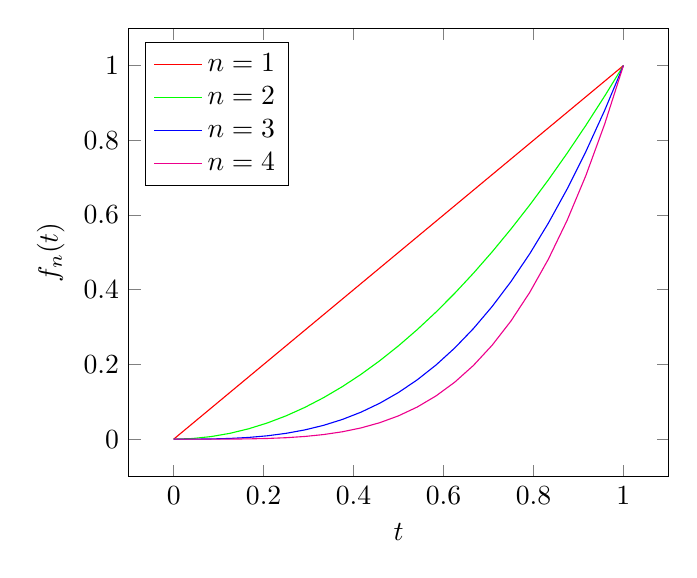
\begin{tikzpicture}
            \begin{axis}[xlabel=$ t $, ylabel=$ f_n(t) $, legend pos=north west]
                \addplot[domain=0:1, color=red] {x};
                    \addlegendentry{$ n=1 $}
                \addplot[domain=0:1, color=green] {x^2};
                    \addlegendentry{$ n=2 $}
                \addplot[domain=0:1, color=blue] {x^3};
                    \addlegendentry{$ n=3 $}
                \addplot[domain=0:1, color=magenta] {x^4};
                    \addlegendentry{$ n=4 $}
            \end{axis}
        \end{tikzpicture}
        \captionof{figure}{The graphs of $ f_n(t) $ over $ [0, 1] $ for $ n = 1,
        2, 3, 4 $.}
    \endgroup
\end{example}
\begin{theorem}{Relationship between Mutual Convergence and Topological
        Equivalence}{convergence-top-equivalence}
    Suppose that $ \left( X, d \right) $ and $ \left( X, d^* \right) $ are
    topologically equivalent. Then,
    \begin{equation}
        \underbrace{\left( x_n \right)_{n=1}^\infty \to x}_{\text{Convergence in
        } \left( X, d \right)} \iff \underbrace{\left( x_n \right)_{n=1}^\infty
        \to x.}_{\text{Convergence in } \left( X, d^* \right)}
    \end{equation}
    \begin{proof}
        Due to the topological equivalence of $ (X, d) $ and $ (X, d^*) $, and
        by \cref{theorem:determining-top-eq}, there exists a scalar $ \lambda >
        0 $ such that
        \begin{equation}
            \frac{1}{\lambda} d^*(x, y) \leq d(x, y) \leq \lambda d^*(x, y)
            \text{ for all } x, y \in X.
        \end{equation}
        \iffforward Suppose that $ \left( x_n \right)_{n=1}^\infty \to x $ as $
        n \to \infty $. Let $ \epsilon > 0 $ be given, and set $ \epsilon^*
        \coloneq \epsilon/\lambda $. By
        \cref{definition:sequence-convergence-metric}, there exists an $ N > 0 $
        such that $ d(x_n, x) < \epsilon^* $ for all $ n > N $. Since $ (X, d) $
        and $ (X, d^*) $ are topologically equivalent,
        \begin{equation}
            \frac{1}{\lambda} d^*(x_n, x) \leq d(x_n, x) < \epsilon^* =
            \frac{\epsilon}{\lambda}.
        \end{equation}
        Since $ \lambda > 0 $, we can multiply through by $ \lambda $:
        \begin{equation}
            d^*(x_n, x) \leq \lambda d(x_n, x) < \epsilon.
        \end{equation}
        Thus, $ d^*(x_n, x) < \epsilon $ for all $ n > N $, so $ \left( x_n
        \right)_{n=1}^\infty \to x $ as $ n \to \infty $ in $ (X, d^*) $.
        \iffbackward A near-identical argument applies: derive convergence in $
        (X, d) $ by assuming convergence in $ (X, d^*) $.
    \end{proof}
\end{theorem}

\lecture{Cauchy Sequences \& More on Convergence}
        {Viewer.aspx?id=0fa218ae-7c44-465c-b963-b09f009bd3ea}{
    Lecture Nine proves the uniqueness of limits, and begins to formalise the
    Cauchy Condition while introducing its various surprising relationships to
    `traditional' convergence. We are also brought to consider the concept of
    pointwise convergence over a sequence of functions.
}{\DTMdisplaydate{2023}{10}{24}{Tuesday}}

\begin{theorem}{Uniqueness of Limits of Convergent
        Sequences}{unique-sequence-limit}
    Let $ (X, d) $ be a metric space, and let $ \left( x_n \right)_{n=1}^\infty
    $ be a convergent sequence in $ (X, d) $ such that $ x_n \to x $, and $ x_n
    \to y $, as $ n \to \infty $. Then, $ x = y $.
    \begin{proof}
        Assume, by way of contradiction, that $ x \neq y $. Thus, $ d(x, y)
        \eqcolon \epsilon < 0 $. Set $ \delta \coloneq \epsilon/2 $. Given that
        $ x_n \to x $ as $ n \to \infty $ there exists an $ N(\delta) > 0 $ such
        that $ d(x_n, x) < \delta = \epsilon/2 $ for all $ n > N $, by
        \cref{definition:sequence-convergence-metric}. Due to the purported
        simultaneous convergence to $ y $, there also exists an $
        \widetilde{N}(\delta) > 0 $ such that $ d(x_n, y) < \delta = \epsilon/2
        $ for all $ n > \widetilde{N} $.

        Thus,
        \begin{equation}
            d(x_n, x) < \delta = \frac{\epsilon}{2} \text{ and }
            d(x_n, y) < \delta = \frac{\epsilon}{2}
        \end{equation}
        for all $ n > M $, where $ M \coloneq \max\left\{ N, \widetilde{N}
        \right\} $. By the triangle inequality,
        \begin{align}
            d(x, y) &\leq d(x, x_n) + d(x_n, y) \\
            &< \delta + \delta \\
            &= \epsilon \text{ for all } n > M.
        \end{align}
        Given that $ \epsilon $ was defined to be equal to $ d(x, y) $, this is
        a contradiction. Therefore, $ x = y $, and the limits are unique.
    \end{proof}
    \centering
    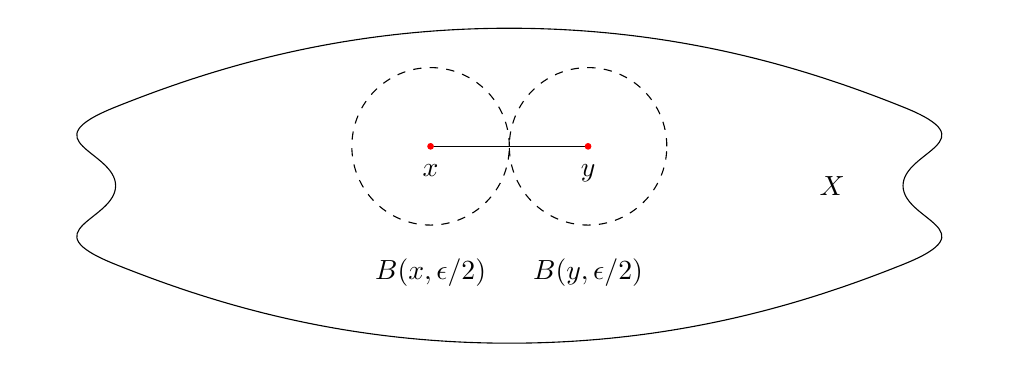
\begin{tikzpicture}
        \coordinate (xpos) at (-1, .5);
        \coordinate (ypos) at (1, .5);
        \pic at (0, 0) {longspace};
        \draw (xpos) -- (ypos);
        \filldraw[red] (xpos) circle (1pt) node[black, below, yshift=-3pt]
            {$ x $};
        \filldraw[red] (ypos) circle (1pt) node[black, below, yshift=-3pt]
            {$ y $};
        \draw[dashed] (xpos) circle (1cm) node[below, yshift=-1.3cm]
            {$ B(x, \epsilon/2) $};
        \draw[dashed] (ypos) circle (1cm) node[below, yshift=-1.3cm]
            {$ B(y, \epsilon/2) $};
        \node at (4.1, 0) {$ X $};
    \end{tikzpicture}
    \captionof{figure}{Given the required sequence convergences, we cannot have
    distinct limits.}
\end{theorem}
\begin{example}{Abstract Infinite Series}{infinite-series}
    We are often concerned with expressions of the form
    \begin{equation}
        S_\infty = \sum_{n=1}^\infty x_n,
    \end{equation}
    where $ S_\infty $ is defined to be the limit of the sequence generated by
    the partial sums
    \begin{equation}
        S_k = \sum_{n=1}^k x_n
    \end{equation}
    as $ k $ approaches infinity. If a metric space $ (X, d) $ supports an
    algebra with a suitable notion of `addition', this idea can be generalised
    to a more abstract setting.
\end{example}
\begin{definition}{Pointwise Convergence}{pointwise-convergence}
    Let $ \left( f_n \right)_{n=1}^\infty $ be a sequence of functions $ f : X
    \to Y $. The function $ f $ is the \emph{pointwise limit} of the function
    sequence if and only if
    \begin{equation}
        \lim_{n \to \infty} f_n{\left( x_0 \right)} = f{\left( x_0 \right)}
        \text{ for any } x_0 \in X.
    \end{equation}
    This equivalence allows us to study convergence in an arbitrary metric space
    by examining convergence in the codomain $ Y $.
\end{definition}
\begin{definition}{The Sequential Characterisation of
        Continuity}{sequential-continuity}
    Let $ f : X \to Y $ be a function from $ (X, d) $ to $ (Y, d^*) $. Then, $ f
    $ is \emph{continuous at} $ x_0 \in X $ if and only if $ f{\left(x_n\right)}
    $ converges to $ f{\left(x_0\right)} $ whenever the sequence generated by $
    x_n $ converges to $ x_0 $.

    The function $ f $ is \emph{continuous} if and only if $ f $ is continuous
    at every point $ x_0 \in X $.
\end{definition}
\begin{definition}{Cauchy Sequence}{cauchy-sequences}
    Let $ \left( x_n \right)_{n=1}^\infty $ be a sequence. Then, $ \left( x_n
    \right)_{n=1}^\infty $ is a \emph{Cauchy sequence} if and only if, for any
    $ \epsilon > 0 $, there exists an $ N > 0 $ such that
    \begin{equation}
        d(x_n, x_m) < \epsilon \text{ for all } n, m > N
    \end{equation}
    The terms of Cauchy sequences grow arbitrarily close, and Cauchy sequences
    need not be convergent.
\end{definition}
\begin{example}{The Cauchy condition does not imply
        convergence}{cauchy-no-convergence}
    Take any sequence of rationals $ p_n/q_n $ for which $ (p_n/q_n)^2 \to 2 $
    as $ n \to \infty $. Note the following:
    \begin{itemize}
        \item $ \left( p_n/q_n \right)_{n=1}^\infty $ is Cauchy;
        \item There is no $ x \in \mathbb{Q} $ such that $ \lim_{n \to
            \infty}{\left( p_n/q_n \right)} = x $, since $ \sqrt{2} \not\in
            \mathbb{Q} $.
    \end{itemize}
    These facts lead to the well-known result regarding the incompleteness of
    the rationals.
\end{example}
\begin{theorem}{Convergence implies Cauchy}{convergence-implies-cauchy}
    Let $ (X, d) $ be a metric space and let $ \left( x_n \right)_{n=1}^\infty $
    be a convergent sequence such that $ \lim_{n \to \infty}{x_n} = x $. Then,
    $ \left( x_n \right)_{x=1}^\infty $ is Cauchy.
    \begin{proof}
        Let $ \epsilon > 0 $ be given, and set $ \delta \coloneq \epsilon/2 $.
        Given that $ \left( x_n \right)_{n=1}^\infty $ is convergent, there
        exists an $ N(\delta) > 0 $ such that $ d(x_n, x) < \delta $ for all $ n
        > N $, according to \cref{definition:sequence-convergence-metric}. By
        the triangle inequality, for all $ n, m > N $,
        \begin{align}
            d(x_n, x_m) &\leq d(x_n, x) + d(x, x_m) \\
            &< \delta + \delta = \epsilon
        \end{align}
        This is precisely the criterion for the Cauchy property on $ \left( x_n
        \right)_{n=1}^\infty $ by \cref{definition:cauchy-sequences}.
    \end{proof}
    This result, combined with the counterexample shown in
    \cref{example:cauchy-no-convergence}, demonstrates that while convergence
    implies Cauchy, Cauchy does not necessarily imply convergence.
\end{theorem}

\lecture{Results on Cauchy Sequences, Subsequences, and Completeness}
        {Sessions/List.aspx\#folderID="494bb17f-0504-4108-b637-b0a700ef131e"}{
    Lecture Ten establishes more useful relationships between the properties of
    a Cauchy sequence and a convergent sequences, and introduces the concept of
    subsequences. The property of completeness is finally defined, along with
    a statement of the Completion Theorem.
}{\DTMdisplaydate{2023}{10}{26}{Tuesday}}

\begin{example}{The Harmonic Series Sequence is not
        Convergent}{harmonic-series-divergent}
    Consider $ (\mathbb{R}, d) $ and the Harmonic series $ \sum_{n=1}^\infty
    (1/n) $. Define a sequence $ \left( S_N \right)_{N=1}^\infty $, such that
    \begin{equation}
        S_N \coloneq \sum_{n=1}^N \frac{1}{n}.
    \end{equation}
    We claim that $ \left( S_N \right)_{N=1}^\infty $ is not convergent; this
    can be shown by considering the contrapositive of the statement given by
    \cref{theorem:convergence-implies-cauchy}: ``not Cauchy'' implies ``not
    convergent''. Consider the difference between $ S_{(2N)} $ and $ S_N $:
    \begingroup
        \setlength\jot{.8em}
        \begin{align}
            \begin{split}
                S_{(2N)} - S_N &= \left( \frac{1}{2N} + \frac{1}{2N-1} + \ldots
                + \frac{1}{N+1} + \frac{1}{N} + \frac{1}{N-1} + \ldots + 1
                \right) -\\ &\left( \frac{1}{N} + \frac{1}{N-1} + \ldots + 1
                \right)
            \end{split}\label{eqn:harmonic-series-1}\\
            &\geq \frac{N}{2N} = \frac{1}{2}\label{eqn:harmonic-series-2}
        \end{align}
    \endgroup
    By \cref{definition:cauchy-sequences}, given an $ \epsilon > 0 $, we need to
    find $ K > 0 $ such that
    \begin{equation}
        \left\vert S_M - S_N \right\vert < \epsilon \text{ for all } M, N > K.
    \end{equation}
    Given \crefrange{eqn:harmonic-series-1}{eqn:harmonic-series-2}, if $ M := 2N
    $, then $ \left\vert S_M - S_N \right\vert > \epsilon $, and the Cauchy
    condition does not hold. By the initial statement, the sequence is therefore
    not convergent.
\end{example}
\begin{definition}{Subsequence}{subsequence}
    Given a metric space $ (X, d) $ containing a sequence $
    \left(x_n\right)_{n=1}^\infty $, a \emph{subsequence} of $ \left( x_n
    \right)_{n=1}^\infty $ is a sequence of elements $ x_{n_1}, x_{n_2}, \ldots,
    x_{n_k}, \ldots $ such that $ n_1 < n_2 < \ldots < n_k < \ldots $.
    Intuitively, we are generating a subsequence by selecting elements from an
    `ambient sequence' while preserving the order of indices.

    \centering
    \begin{tikzpicture}
        \pic at (0, 0) {longspace};
        \node at (4.1, 0) {$ X $};
        \begin{scope}[every node/.style={black, below, yshift=-3pt}]
            \begin{scope}[every path/.style={red}]
                \filldraw (-4, 0) circle (1pt) node {$ x_1 $};
                \filldraw (-2, -.5) circle (1pt) node {$ x_3 $};
                \filldraw (1, 0) circle (1pt) node {$ x_6 $};
                \filldraw (2, 1) circle (1pt) node {$ x_7 $};
            \end{scope}
            \begin{scope}[every path/.style={blue}]
                \filldraw (-3, .5) circle (1pt) node {$ x_2 $};
                \filldraw (-1, 1) circle (1pt) node {$ x_4 $};
                \filldraw (0, -.5) circle (1pt) node {$ x_5 $};
                \filldraw (3, -.5) circle (1pt) node {$ x_8 $};
            \end{scope}
        \end{scope}
    \end{tikzpicture}
    \captionof{figure}{An ambient sequence (red and blue points) generated by $
    x_n $ over $ n = 1, \ldots, 8 $, and a subsequence (blue points only) $
    x_{n_k} $ with $ k = 2, 4, 5, 8 $.}
\end{definition}
\begin{theorem}{Convergence in Subsequences}{subsequence-convergence}
    If $ \left( x_n \right)_{n=1}^\infty $ is a sequence in $ (X, d) $ such that
    $ \lim_{n \to \infty}{x_n} = x $, then any subsequence of $ \left( x_n
    \right)_{n=1}^\infty $ shares the limit. The converse also holds; this
    induces a useful contraposition test for non-convergence: if any subsequence
    is not convergent, then the ambient sequence is neither convergent.
\end{theorem}
\begin{example}{Determining Divergence by Testing
        Subsequences}{subsequence-divergence-contraposition}
    Consider he sequence generated by $ x_n \coloneq \left( \pm x \right)^n $ in
    $ \mathbb{R} $. Then consider the subsequences generated by extracting terms
    at even and odd indices and examine their respective limits:
    \begin{alignat}{4}
        n_1 = 1,\, n_2 = 3,\, n_3 = 5,\, \ldots & \quad\mapsto\quad &&
            (-1, -1, -1, \ldots) && \quad\to\quad -1 && \quad(\text{as } n \to
            \infty) \\
        n_1 = 2,\, n_2 = 4,\, n_3 = 6,\, \ldots & \quad\mapsto\quad &&
            (1, 1, 1, \ldots) && \quad\to\quad 1 && \quad(\text{as } n \to
            \infty)
    \end{alignat}
    By the contraposition test described by
    \cref{theorem:subsequence-convergence}, we can see immediately that $ \left(
    x_n \right)_{n=1}^\infty $ diverges, given that its subsequences do not
    converge to a consistent limit.
\end{example}
\begin{definition}{Completeness}{completeness}
    Let $ (X, d) $ be a metric space. Then, $ X $ is \emph{complete} if and only
    if any Cauchy sequence converges to a point in $ X $. We may assume that $
    (\mathbb{R}, d) $ is complete.

    If a sequence is Cauchy, and its resident metric space is complete, then the
    sequence is convergent. To show that a space is \emph{not complete}, we must
    find a Cauchy sequence in the space which does not converge to another point
    in the space.

    \centering
    \begin{tikzpicture}
        \node {\fbox{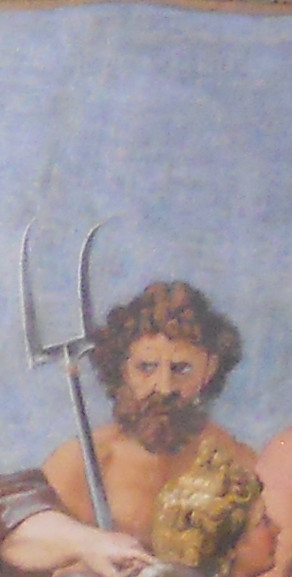
\includegraphics[angle=-90]{pluto}}};
        \node[white, rotate=-10] at (1.5, .8) {\large Cauchy};
        \node[white, rotate=-20] at (1.5, 0) {\large Complete};
    \end{tikzpicture}
    \captionof{figure}{\href{https://en.wikipedia.org/wiki/Bident\#In\_art}%
        {Pluto}, the Greek God of Convergence, brandishing his topological
        bident}
\end{definition}
\begin{theorem}{The Completion Theorem}{completion-theorem}
    Let $ (X, d) $ be a metric space. There is a metric space $ (X^*, d^*) $ and
    an isometry $ \psi \colon X \to X^* $ such that the following properties
    hold:
    \begin{itemize}
        \item $ X^* $ is complete (c.f. \cref{definition:completeness}); and
        \item $ \psi(X) $ is dense in $ X^* $ (c.f. \cref{definition:density}).
    \end{itemize}
    $ X^* $ is called a \emph{completion} of $ X $; all completions of $ X $ are
    isometric to $ X^* $.
    \begin{proof}
        Proof sketch:
        \begin{enumerate}
            \item If $ X $ is already complete, we can set $ X^* \coloneq X $
                and $ \psi(x) \coloneq x $ and finish. Therefore, we assume that
                $ X $ is not complete.
            \item Collate the set of all Cauchy sequences in $ X $, and denote
                the set as $ \mathcal{G}(X) $. This set is trivially nonempty:
                for the degenerate case of a singleton $ X = \{x\} $, we can
                extract the Cauchy sequence $ (x, x, \ldots) $.
            \item Define an equivalence relation $ \sim $ on $ \mathcal{G}(X) $
                such that
                \begin{equation}
                    \left( x_n \right) \sim \left( y_n \right) \iff
                    \lim_{n \to \infty}{d\left( x_n, y_n \right)} = 0
                    \text{ for all sequences in } \mathcal{G}(X).
                \end{equation}
            \item Construct the set of all equivalence classes under the $ \sim
                $ relation: the quotient set $ \cauchyquotient $.
            \item Extend the metric $ d $ on $ X $ to the metric $ d^* $ on $
                X^* $ by defining a map $ \widetilde{d} \colon \cauchyquotient~%
                \to \mathbb{R} $ such that
                \begin{equation}
                    \left(\left[\left( x_n \right)\right], \left[\left( y_n
                    \right)\right]\right) \mapsto \lim_{n \to
                    \infty}{d\left( x_n, y_n \right)} \in \mathbb{R}.
                \end{equation}
            \item Define the isometry map $ \psi \colon X \to X^* $ such that
                \begin{equation}
                    x \mapsto \left[ (x)_{n=1}^\infty \right] \in
                    \cauchyquotient\text{ where } \left[ (x)_{n=1}^\infty
                    \right] = (x, x, \ldots),
                \end{equation}
                and prove that $ \psi $ is an isometry.
            \item Show that $ \overline{\psi{(X)}} = \cauchyquotient= X^* $,
                thereby confirming density.
            \item Show that any Cauchy sequence in $ \cauchyquotient $ converges
                to a common limit in the same quotient set, and prove
                uniqueness.
        \end{enumerate}
        The detailed proof is completed in Section 1.5 of
        \autocite{Shirali:2006}.
    \end{proof}
\end{theorem}
\begin{theorem}{A real-valued vector space is complete under the sup-metric}
            {real-vector-sup-complete}
    The space $ \left( \mathbb{R}^k, d_\infty \right) $ where $ k \geq 2 $ is
    complete.
    \begin{proof}
        By \cref{definition:completeness}, and in the same vein as
        \cref{theorem:completion-theorem}, we take an arbitrary Cauchy sequence
        $ \left( \vec{x}_n \right)_{n=1}^\infty $ from $ \left( \mathbb{R}^k,
        d_\infty \right) $, and let $ \epsilon > 0 $ be given. Since $ \left(
        \vec{x}_n \right)_{n=1}^\infty $ is Cauchy,
        there exists an $ N(\epsilon) > 0 $ such that, for all $ n, m > N $,
        \begin{alignat}{2}
            d_\infty\left( \vec{x}_n, \vec{x}_m \right) &= \max_{1 \leq i \leq
            k}\left\{ \left\vert x_i^{(n)} - x_{i}^{(m)} \right\vert
            \right\}\quad &&\text{[\Cref{definition:canon-metrics}]}\\
            &< \epsilon &&\text{[\Cref{definition:cauchy-sequences}]}
        \end{alignat}
        Given that $ \mathbb{R} $ is axiomatised to be complete, each real
        subsequence converges to a real limit. Since we know the limit to exist,
        we can construct a candidate limit $ \vec{x} $ to be the component-wise
        limits, as pictured below.
        \begin{equation*}
            \renewcommand\arraystretch{1.8}
            \begin{matrix}
                \vec{x}_1 & \vline & \Big( & x_1^{(1)}, & x_1^{(2)}, & \ldots,
                    & x_1^{(k)} & \Big) \\
                \vec{x}_2 & \vline & \Big( & x_2^{(1)}, & x_2^{(2)}, & \ldots,
                    & x_2^{(k)} & \Big) \\
                \vdots & \vline & & \big\downarrow & \big\downarrow & \ddots &
                    \big\downarrow & \\
                \color{red}{\vec{x}} & \vline & \Big( & {\color{red}x_1}, &
                    {\color{red}x_2}, & \ldots, & {\color{red}x_k} & \Big) &
                    \begin{rcases}\vphantom{\Big)}\end{rcases}\,\,N(\epsilon)
            \end{matrix}
        \end{equation*}

        After the index $ N $, $ \vec{x}_n $ and $ \vec{x}_m $ are sufficiently
        close by the $ d_\infty $ metric; that is, $ \vec{x} \in \mathbb{R}^k $
        is composed of the component-wise limits of $ \vec{x}_i $ for $ i \in
        \mathbb{N} $. We can use \cref{theorem:vector-space-convergence} to show
        that the candidate limit $ \vec{x} $ is valid, given that the coordinate
        sequences converge component-wise (by construction of $ \vec{x} $).

        Thus, any arbitrary Cauchy sequence $ \left( \vec{x}_n
        \right)_{n=1}^\infty \in \left( \mathbb{R}^k \right)^\mathbb{N} $
        converges to $ \vec{x} \in \mathbb{R}^k $, so $ \left( \mathbb{R}^k,
        d_\infty \right) $ is complete by \cref{definition:completeness}.
    \end{proof}
\end{theorem}

\lecture{Generalising Continuity}
        {Viewer.aspx?id=227c74d2-ed70-4345-bed6-b0ad00abd4d4}{
    Lecture Eleven introduces a general form of continuity according to the $
    \epsilon $--$ \delta $ definition and hence motivates five superficially
    different, albeit equivalent, notions of a continuous map in terms of highly
    abstract open and closed sets. The sets of bounded and continuous functions
    are revisited with greater care, and an example helps to illustrate $ B(X,
    Y) $ with the $ d_\infty $ metric.
}{\DTMdisplaydate{2023}{11}{7}{Tuesday}}

\begin{definition}{Inverse Image (Traditional Interpretation)}
        {inverse-image-traditional}
    Consider $ f \colon X \to Y $, and let $ A \subseteq Y $. Then, the
    \emph{inverse image} of $ A $ is defined as
    \begin{equation}
        f^{-1}{(A)} \coloneq \left\{ x \in X \colon f(x) \in A \right\}.
    \end{equation}
\end{definition}
\begin{definition}{Inverse Image (Fibreoptic Interpretation)}
        {inverse-image-fibre}
    Following from \cref{definition:inverse-image-traditional}, we can define a
    \emph{fibre} of $ y $ to be the inverse image of the singleton set $ \{ y \}
    \subseteq Y $, denoted $ F_y $:
    \begin{equation}
        F_y \coloneq \left\{ x \in X \colon f(x) = y \right\}.
    \end{equation}
    Then, the \emph{inverse image} of $ A $ is the union over all fibres of the
    singletons in $ A $:
    \begin{equation}
        f^{-1}{(A)} = \bigcup_{y \in A} F_y.
    \end{equation}
\end{definition}
\begin{definition}{Continuity on the Real Line}{real-continuity}
    A function $ f \colon \mathbb{R} \to \mathbb{R} $ is \emph{continuous} if
    and only if, for all $ \epsilon > 0 $ there exists a $ \delta{(\epsilon)} >
    0 $ such that
    \begin{equation}
        \left\vert x - x_0 \right\vert < \delta \implies \left\vert f{(x)} -
        f{\left(x_0\right)} \right\vert < \epsilon.
    \end{equation}
    This is the least abstract, yet formally correct, definition of continuity,
    as it applies only to the set of real numbers. Over the next set of
    definitions, we define increasingly abstract---albeit equivalent---notions
    of \emph{continuity in a metric space}.
\end{definition}
\begin{definition}{Continuity in an Abstract Metric Space}{continuity}
    Let $ (X, d) $ and $ (Y, \widetilde{d}) $ be metric spaces. The function $ f
    \colon X \to Y $ is continuous at $ x_0 \in X $ if any of the following
    equivalent definitions holds:
    \begin{enumerate}
        \item \textbf{(Analytic Definition)} For any $ \epsilon > 0 $, there
            exists a $ \delta > 0 $ such that $
            \widetilde{d}\left(f\left(x\right), f\left(x_0\right)\right) <
            \epsilon $ whenever $ d\left(x, x_0\right) < \delta $.
        \item \textbf{(Open Ball Definition)} For any $ \epsilon > 0 $, there
            exists a $ \delta > 0 $ such that $ f\left(B\left(x_0,
            \delta\right)\right) \subseteq B\left(f\left(x_0,
            \epsilon\right)\right) $. See \cref{fig:open-ball-continuous}.
        \item \textbf{(Open Set with Ball Definition)} For any open set $ V
            \subseteq Y $ with $ f\left( x_0 \right) \in V $, there exists a
            \emph{ball} $ B \subseteq X $ such that $ x_0 \in B $ and $ f(B)
            \subseteq V $.
        \item \textbf{(Purely Topological Definition)} For any open set $ V
            \subseteq Y $ with $ f\left(x_0\right) \in V $, there exists an
            \emph{open set} $ U \subseteq X $ with $ x_0 \in U $ and $ f(U)
            \subseteq V $.
        \item \textbf{(Sequence Definition)} For any sequence $ \left( x_n
            \right)_{n=1}^\infty $ with $ \lim_{n \to \infty} x_n = x_0 $, the
            sequence generated by $ f\left( x_n \right) $ is such that $ \lim_{n
            \to \infty}f\left(x_n\right) = f\left(x_0\right) $.
    \end{enumerate}
    To prove the equivalence between these definitions, we need to demonstrate
    the following cycle of implications:
    \begin{equation}
        \text{\#1} \implies \text{\#2} \implies \text{\#3} \implies \text{\#4}
        \implies \text{\#5} \implies \text{\#1}.
    \end{equation}
    In particular, we will show that $ \text{\#4} \implies \text{\#5} $
    (\cref{theorem:seq-top-continuity}), followed by $ \text{\#5} \implies
    \text{\#1} $ (\cref{theorem:top-anal-continuity}). The equivalences of
    statements \#1 through \#4 can be trivially established through previously
    established results on the connexions between open balls and open sets, such
    as those enumerated throughout \cref{sec:topology-results}.

    \centering
    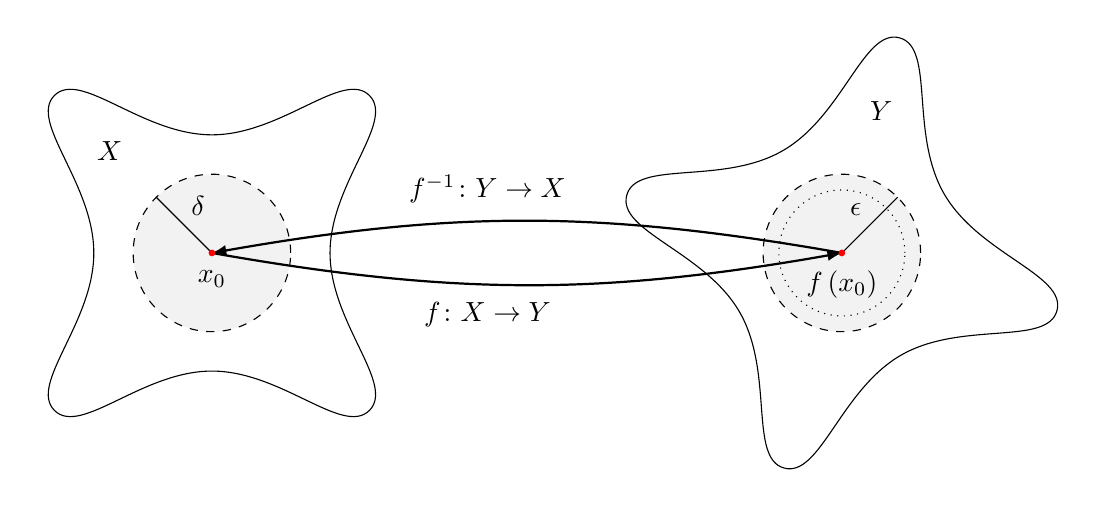
\begin{tikzpicture}
        \coordinate (leftball) at (-4, 0);
        \coordinate (rightball) at (4, 0);
        \pic at (leftball) {squarespace};
        \node at (-5.3, 1.3) {$ X $};
        \pic[rotate=30] at (rightball) {squarespace};
        \node at (4.5, 1.8) {$ Y $};
        \draw[fill=ballfill, dashed] (leftball) circle (1cm);
        \draw[fill=ballfill, dashed] (rightball) circle (1cm); % B(f(x0), e))
        \draw[fill=ballfill, dotted] (rightball) circle (.8cm); % f(B(x0, d))
        \draw[thick, latex-] (leftball) to [bend left=10] (rightball)
            node[above, yshift=.5cm, xshift=-.5cm, pos=.5]
            {$ f^{-1} \colon Y \to X $};
        \draw[thick, latex-] (rightball) to [bend left=10] (leftball)
            node[below, yshift=-.5cm, xshift=-.5cm, pos=.5]
            {$ f \colon X \to Y $};
        \draw (leftball) -- ++(135:1cm) node[above, pos=.5, xshift=5pt]
            {$ \delta $};
        \draw (rightball) -- ++(45:1cm) node[above, pos=.5, xshift=-5pt]
            {$ \epsilon $};
        \begin{scope}[every path/.style={red}, every node/.style={black, below,
                yshift=-3pt}]
            \filldraw (leftball) circle (1pt) node {$ x_0 $};
            \filldraw (rightball) circle (1pt) node {$ f\left(x_0\right) $};
        \end{scope}
    \end{tikzpicture}
    \captionof{figure}{An open ball $ B\left(x_0, \delta\right) \subseteq X $
    with two open balls in $ Y $ such that $ f\left(B\left( x_0, \delta
    \right)\right) \subseteq B\left(f\left(x_0\right), \epsilon\right) \subseteq
    Y $, marked by dotted, dashed, and solid paths
    respectively.}\label{fig:open-ball-continuous}
\end{definition}
\begin{theorem}{The sequential statement of continuity follows from the
        topological definition}{seq-top-continuity}
    Let $ x_0 \in X $ and let $ \left( x_n \right)_{n=1}^\infty $ be a sequence
    in $ X $ such that $ \lim_{n \to \infty} x_n = x_0 $. If, for any open set $
    V \subseteq Y $ with $ f\left( x_0 \right) \in V$, there exists an open set
    $ U \subseteq X $ with $ x_0 \in U $ and $ f(U) \subseteq V $, then the
    sequence generated by $ f\left( x_n \right) $ is such that $ \lim_{n \to
    \infty} f\left(x_n\right) = f\left(x_0\right) $.
    \begin{proof}
        Take an arbitrary open set $ V \subseteq Y $ with $ f\left(x_0\right)
        \in V $; thus, there exists an open set $ U \subseteq X $ such that $
        x_0 \in U $ and $ f(U) \subseteq V $. Given that $ U $ is open, there
        exists an open ball by \cref{theorem:openness-open-balls}: $ \exists
        \epsilon > 0 $ such that $ B\left(x_0, \epsilon\right) \subseteq U $. As
        $ \left(x_n\right)_{n=1}^\infty $ tends to $ x_0 $, we can find an index
        point $ N > 0 $ such that $ d\left(x_n, x_0\right) < \epsilon $ for all
        $ n > N $ (by \cref{definition:sequence-convergence-metric}).

        Thus, $ f\left(x_n\right) \in f(U) \subseteq V $ for all $ n > N $.
        Given that $ V $ was chosen arbitrarily, any sequence generated by $
        f\left(x_n\right) $ must converge to $ f\left(x_0\right) $.
    \end{proof}
\end{theorem}
\begin{theorem}{The analytical statement of continuity follows from the
        sequential definition}{top-anal-continuity}
    For any sequence $ \left(x_n\right)_{n=1}^\infty $ such that $ \lim_{n \to
    \infty} x_n = x_0 $, if the sequence $
    \left(f\left(x_n\right)\right)_{n=1}^\infty $ is such that $ \lim_{n \to
    \infty} f\left(x_n\right) = f\left(x_0\right) $, then given an $ \epsilon >
    0 $, there exists a $ \delta > 0 $ such that $ d\left(f(x),
    f\left(x_0\right)\right) < \epsilon $ whenever $ \widetilde{d}\left(x,
    x_0\right) $.
    \begin{proof}
        We will prove this using contraposition (modus tollens); the argument is
        visualised below with the premise $ P $ and conclusion $ Q $, to argue
        that $ \lnot Q \implies \lnot P $.

        \begingroup
            \renewcommand\fboxsep{.8em}
            \begin{align*} % Great test of your editor's syntax highlighting!
                \underbrace{\mathrm{\fbox{\parbox{.42\linewidth}{
                    For an arbitrary sequence $ \left(x_n\right)_{n=1}^\infty $
                    such that $ x_n \to x_0 $ as $ n \to \infty $, the sequence
                    $ f\left( x_n \right) \to f\left( x_0 \right) $ as $ n \to
                    \infty $.
                }}}}_{\text{Premise } P}&\implies
                \underbrace{\mathrm{\fbox{\parbox{.42\linewidth}{
                    For any $ \epsilon > 0 $, there exists a $ \delta > 0 $ such
                    that $ d\left( f(x), f\left( x_0 \right) \right) < \epsilon
                    $ whenever $ \widetilde{d}\left( x, x_0 \right) $.
                }}}}_{\text{Conclusion } Q} \\
                &\tikz\node[rotate=90, minimum size=1cm] {$ \iff $}; \\
                \underbrace{\mathrm{\fbox{\parbox{.42\linewidth}{
                    There exists some $ \epsilon > 0 $ such that, for all $
                    \delta > 0 $, $ \widetilde{d}\left( f(x), f\left(x_0\right)
                    \right) \geq \epsilon $ for some $ x \in X $ with $ d\left(
                    x, x_0 \right) < \delta $.
                }}}}_{\text{Negated Conclusion } \lnot Q}&\implies
                \underbrace{\mathrm{\fbox{\parbox{.42\linewidth}{
                    There exists a sequence $ \left(x_n\right)_{n=1}^\infty $
                    such that $ x_n \to x_0 $ as $ n \to \infty $, but $ f\left(
                    x_n \right) \not\to f\left( x_0 \right) $.
                }}}}_{\text{Negated Premise } \lnot P}
            \end{align*}
        \endgroup

        We will assume $ \lnot Q $ and derive $ \lnot P $. For each $ n \in
        \mathbb{N} $, define the set
        \begin{equation}
            A_n \coloneq \left\{ x^\prime \in X \colon d\left(x^\prime,
            x_0\right) < \frac{1}{n} \,\land\, \widetilde{d}\left(
            f\left(x^\prime\right), f\left(x_0\right) \right) \geq \epsilon
            \right\}.
        \end{equation}
        By the assumption of $ \lnot Q $, $ A_n $ is non-empty for all $ n \in
        \mathbb{N} $. Thus, for each $ n $, pick an element $ x_n \in A_n $ and
        note that $ \lim_{n \to \infty} x_n = x_0 $, but $ \lim_{n \to \infty}
        \widetilde{d}\left( f\left(x_n\right), f\left(x_0\right) \right) \geq
        \epsilon $, so the sequence generated by $ f\left(x_n\right) $ does not
        converge to $ f\left(x_0\right) $. Hence, $ P $ does not hold, as
        required.
    \end{proof}
\end{theorem}

\lecture{Applications of Continuity}
        {Viewer.aspx?id=67becd92-a94f-4318-a4ae-b0af00ac252a}{
    Lecture Twelve reframes much of the theoretical discussion around continuity
    into a more applied context, in which the equivalent definitions of a
    continuous map are considered in bounded and continuous function spaces.
    Some remarks are made in the realm of closed sets, particularly with regard
    to the concept of \emph{global continuity}, where we have previously
    focussed on manipulations with open sets to show \emph{local} continuity.
}{\DTMdisplaydate{2023}{11}{9}{Thursday}}

\begin{definition}{Global continuity (by way of local continuity)}
        {global-continuity-local}
    Let $ f \colon X \to Y $. Then, $ f $ is \emph{globally continuous} if and
    only if it is (locally) continuous, by \cref{definition:continuity}, at
    every point $ x_0 \in X $.
\end{definition}
\begin{definition}{Global continuity (topological perspective)}
        {global-continuity-topology}
    If $ V \subseteq Y $ is open, then $ f $ is \emph{globally continuous} if
    and only if $ f^{-1}(V) \subseteq X $ is also open; this is justified
    formally by \cref{theorem:global-continuity-open-preimage}. We can
    eventually restate this definition in terms of a closed set $ F \subseteq Y
    $, justified by justified by
    \cref{theorem:global-continuity-closed-preimage}:
    \begin{align}
        f \text{ is globally continuous}
        &\iff V \in T_e \implies f^{-1}(V) \in T_d \\
        &\iff f^{-1}(F) \text{ is closed.}
    \end{align}

    \centering
    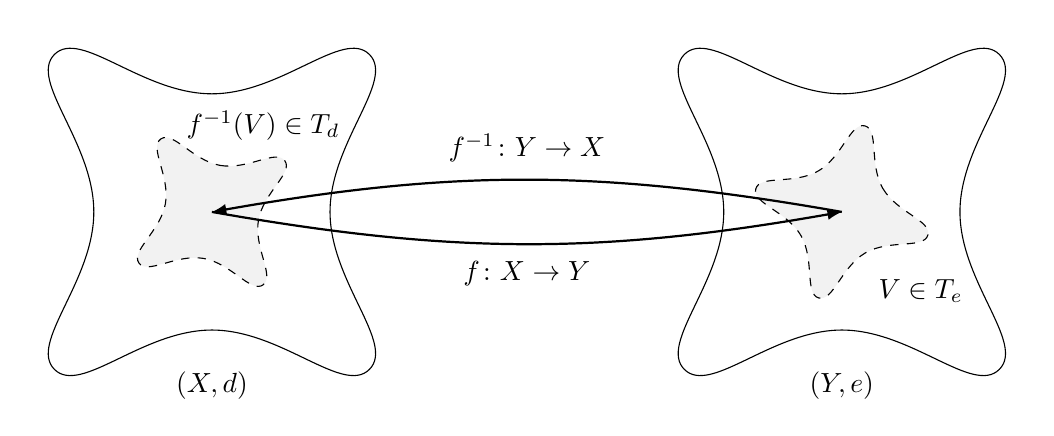
\begin{tikzpicture}
        \coordinate (leftspace) at (-4, 0);
        \coordinate (rightspace) at (4, 0);
        \pic at (leftspace) {squarespace};
        \pic at (rightspace) {squarespace};
        \begin{scope}[every node/.style={scale=.4},
                every path/.style={fill=ballfill, dashed}]
            \pic[rotate=80] at (leftspace) {squarespace};
            \pic[rotate=30] at (rightspace) {squarespace};
        \end{scope}
        \node[below of=leftspace, yshift=-1.2cm] {$ (X, d) $};
        \node[below of=rightspace, yshift=-1.2cm] {$ (Y, e) $};
        \draw[thick, latex-] (leftspace) to [bend left=10] (rightspace)
            node[above, yshift=.5cm, pos=.5] {$ f^{-1} \colon Y \to X $};
        \draw[thick, latex-] (rightspace) to [bend left=10] (leftspace)
            node[below, yshift=-.5cm, pos=.5] {$ f \colon X \to Y $};
        \node[right of=rightspace, yshift=-1cm] {$ V \in T_e $};
        \node[right of=leftspace, yshift=1.1cm, xshift=-1em]
            {$ f^{-1}(V) \in T_d $};
    \end{tikzpicture}
    \captionof{figure}{Considering the membership of the pre-image of $ V $
    under $ f $ in the topology of the domain space, versus membership in the
    topology of the codomain space, can reveal $ f $ to be a globally continuous
    map.}
\end{definition}
\begin{example}{Global continuity in the plane}{global-continuity-plane}
    Consider $ f \colon \mathbb{R}^2 \to \mathbb{R} $ such that $ (x, y) \mapsto
    x^2 + e^y $ and a curve $ \Gamma $ such that
    \begin{equation}
        \Gamma \coloneq \left\{ (x, y) \in \mathbb{R}^2 \colon f(x, y) = 1
        \right\}.
    \end{equation}

    % Some manual positioning is necessary here, since the two plots need to be
    % aligned along non-plot boundaries (but rather their internal axis
    % y-positions).
    \begingroup
        \tikzset{external/export=true}
        \centering
        \hspace*{-2em}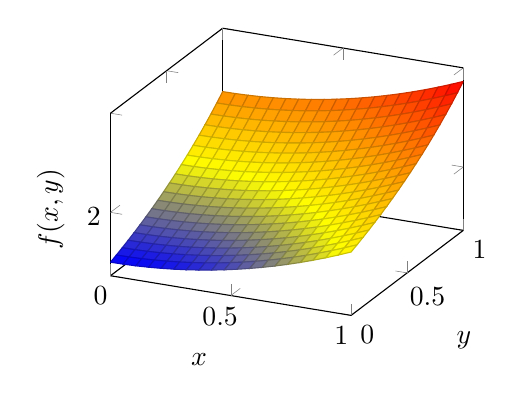
\begin{tikzpicture}
            \begin{axis}[xlabel=$ x $, ylabel=$ y $, zlabel={$ f(x, y) $},
                width=.5\linewidth]
                \addplot3[mesh, samples=20, domain=0:1, mark=none, surf]
                    {x^2 + e^y};
            \end{axis}
        \end{tikzpicture}\qquad
        \raisebox{2em}{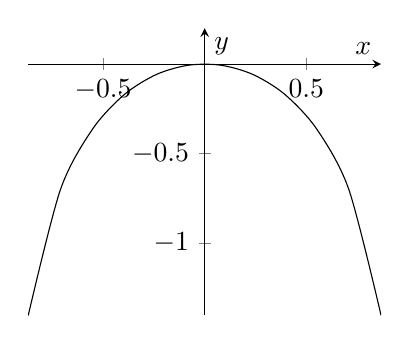
\begin{tikzpicture}
            \begin{axis}[xlabel=$ x $, ylabel=$ y $, axis lines=middle, ymax=.2,
                width=.5\linewidth]
                \addplot[samples=20, smooth, domain=-1.5:1.5,
                    unbounded coords=jump] {ln(1-x^2)};
            \end{axis}
        \end{tikzpicture}}
        \captionof{figure}{The mesh $ z = f(x, y) $ with the level set $ \Gamma
        $.}
    \endgroup

    By \cref{definition:global-continuity-topology} it is easy to verify that $
    \Gamma $ is closed in $ \mathbb{R}^2 $: given that $ f $ is globally
    continuous, and given that $ \{ 1 \} $ is closed---as are all
    singletons---its inverse image $  $ is
    also closed. Since $ \Gamma = f^{-1}\left(\left\{1\right\}\right) $, $
    \Gamma $ is closed.
\end{example}
\begin{theorem}{Constant functions are globally
        continuous}{constant-global-continuity}
    Let $ f \colon X \to Y $ be such that $ x \mapsto k $, where $ k $ is fixed.
    Then, $ f $ is continuous.
    \begin{proof}
        The singleton $ \{ k \} $ is known to be closed, and the entire domain
        space $ f^{-1}\left(\left\{ k \right\}\right) = X $ is known to be
        clopen, and thus closed. Hence, by
        \cref{definition:global-continuity-topology}, $ f $ is continuous.
    \end{proof}
\end{theorem}
\begin{theorem}{Continuity is preserved under function
        composition}{continuity-preserved-composition}
    Let $ f \colon X \to Y $ and $ g \colon Y \to Z $ be a pair of continuous
    functions. Then, $ g \fcomp f \colon X \to Z $ is also continuous.
    \begin{proof}
        Let $ V \subseteq Z $ be open. Given that $ f $ and $ g $ are
        continuous, $ g^{-1}(V) \subseteq Y $ and $ f^{-1}\left(g^{-1}(V)\right)
        \subseteq X $ are open in their respective spaces, by
        \cref{definition:global-continuity-topology}. It is known from set
        theory that
        \begin{equation}
            \left(g \fcomp f \right)^{-1}(V) = f^{-1}\left(g^{-1}(V)\right),
        \end{equation}
        and hence the composition is continuous. It follows immediately that $ g
        \fcomp f $ is continuous.
    \end{proof}
\end{theorem}
\begin{example}{Continuous Composition of Non-Continuous Constituents}
        {cont-comp-non-cont}
    Consider the pair of functions $ f $ and $ g $ from $ \mathbb{R} $ to $ [-1,
    1] $ such that
    \begin{align}
        f(t) &\coloneq \begin{cases}
            1 \text{ if } t \geq 0; \\
            -1 \text{ otherwise.}
        \end{cases} \\
        g(t) &\coloneq 0 \text{ for all } t \in \mathbb{R}.
    \end{align}
    $ f $ is clearly non-continuous. Despite that, $ (g \fcomp f)(t) = 0 $ for
    all $ t \in \mathbb{R} $, which is continuous. Therefore, continuity on a
    composition does not generally imply continuity on the individual
    components.
\end{example}
\begin{theorem}{Global continuity is equivalent to open
        pre-images}{global-continuity-open-preimage}
    Let $ f \colon X \to Y $. Then, $ f $ is globally continuous if and only if,
    for any open set $ V \subseteq Y $, $ f^{-1}(V) $ is open in $ X $.
    \begin{proof}
        \iffforward \textbf{(Using fibres.)} Suppose that $ f \colon X \to Y $
        is globally continuous, and consider an open set $ V \subseteq Y $.  If
        $ V = \emptyset $, then $ f^{-1}(V) = \emptyset $, and we are done,
        since the empty set is open.  Assuming that $ V \neq \emptyset $, take $
        y \in V $, and note the multiple possibilities for the nature of $ y $:
        \begin{itemize}
            \item If $ y \not\in f(X) $, then $ F_y = \emptyset $, and we are
                done.
            \item If $ y \in f(X) $, then $ F_y \neq \emptyset $; that is, there
                exists an $ x \in X $  such that $ f(x) = y $. Given that $ V $
                is open and $ f $ is continuous, by
                \cref{theorem:openness-open-balls}, there exists an open ball $
                B \subseteq X $ such that $ x \in B $ and $ f(B) \subset V $.
                Take the union over all such balls to acquire the entire inverse
                image of $ V $ in $ X $:
                \begin{equation}
                    f^{-1}(V) = \bigcup_{\substack{y \in V \\ F_y \neq
                        \emptyset}} F_y = \bigcup_{x \in f^{-1}(V)} B_x
                \end{equation}
        \end{itemize}
        By \cref{theorem:open-union-open} with \cref{theorem:open-ball-open}, $
        f^{-1}(V) $ is a union of open balls, and is therefore open, as
        required. (This is an example of an \emph{open cover}.)

        \iffbackward \textbf{(Using epsilon--deltas.)} Conversely, suppose that
        $ f^{-1}(V) \subseteq X $ is open for all open sets $ V \subseteq V $.
        Take an $ x \in X $, and note that $ B\left(f(x), \epsilon\right) $ is
        open in $ Y $, and $ f^{-1}\left(B\left(f(x), \epsilon\right)\right) $
        is open in $ X $. Since $ x \in f^{-1}\left(B\left(f(x),
        \epsilon\right)\right) $, there exists a $ \delta(\epsilon) > 0 $ such
        that $ B(x, \delta) \subseteq f^{-1}\left(B\left(f(x),
        \epsilon\right)\right) $. Hence, $ f $ is continuous at $ x $. Given
        that $ x \in X $ was chosen arbitrarily, $ f $ is globally continuous.
    \end{proof}

    \centering
    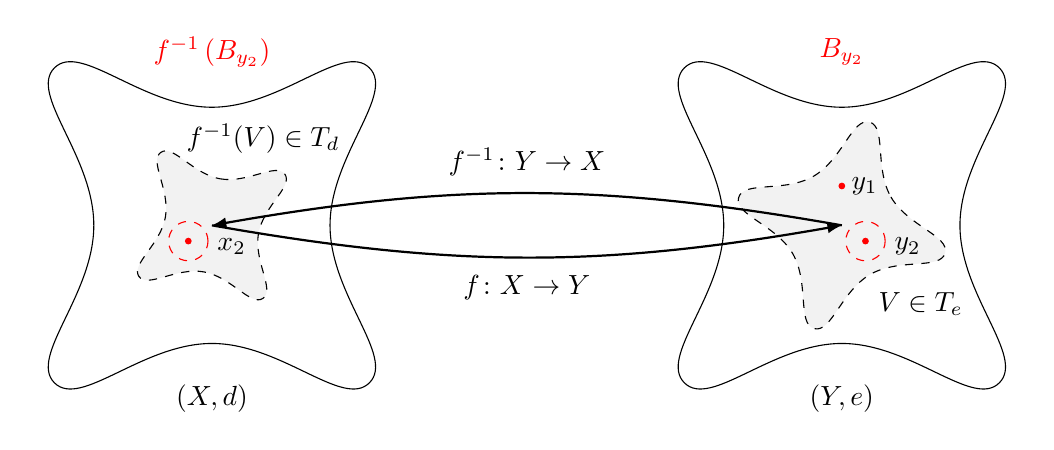
\begin{tikzpicture}
        \coordinate (leftspace) at (-4, 0);
        \coordinate (rightspace) at (4, 0);
        \coordinate (y1point) at (4, .5);
        \coordinate (y2point) at (4.3, -.2);
        \coordinate (x2point) at (-4.3, -.2);
        \pic at (leftspace) {squarespace};
        \pic at (rightspace) {squarespace};
        \begin{scope}[every node/.style={scale=.4},
                every path/.style={fill=ballfill, dashed}]
            \pic[rotate=80] at (leftspace) {squarespace};
            \pic[rotate=30, scale=1.2] at (rightspace) {squarespace};
        \end{scope}

        \filldraw[red] (y1point) circle (1pt) node[right, black] {$ y_1 $};
        \foreach \pt/\name in {x2point/x, y2point/y}{
            \draw[dashed, red] (\pt) circle (.25cm); % Open ball
            \filldraw[red] (\pt) circle (1pt) node[right, black, xshift=7pt,
                yshift=-2pt] {$ \name_2 $}; % Point
        }

        \node[red, above of=leftspace, yshift=1.2cm]
            {$ f^{-1}\left(B_{y_2}\right) $};
        \node[red, above of=rightspace, yshift=1.2cm] {$ B_{y_2} $};
        \node[below of=leftspace, yshift=-1.2cm] {$ (X, d) $};
        \node[below of=rightspace, yshift=-1.2cm] {$ (Y, e) $};

        \draw[thick, latex-] (leftspace) to [bend left=10] (rightspace)
            node[above, yshift=.5cm, pos=.5] {$ f^{-1} \colon Y \to X $};
        \draw[thick, latex-] (rightspace) to [bend left=10] (leftspace)
            node[below, yshift=-.5cm, pos=.5] {$ f \colon X \to Y $};
        \node[right of=rightspace, yshift=-1cm] {$ V \in T_e $};
        \node[right of=leftspace, yshift=1.1cm, xshift=-1em]
            {$ f^{-1}(V) \in T_d $};
    \end{tikzpicture}
    \captionof{figure}{Mapping $ V $ with open balls in $ Y $, and their
    respective pre-images in $ X $.}
\end{theorem}
\begin{theorem}{Global continuity is equivalent to closed
        pre-images}{global-continuity-closed-preimage}
    Let $ f \colon X \to Y $. Then, $ f $ is globally continuous if and only if,
    for any closed set $ F \subseteq Y $, $ f^{-1}(F) $ is closed in $ X $.
    \begin{proof}
        Recall from \cref{theorem:global-continuity-open-preimage} that the
        property of global continuity on $ f $ is equivalent to the openness of
        $ V \subseteq Y $ implying the openness of $ f^{-1}(V) \subseteq X $.

        \iffforward Suppose that $ F \subseteq Y $ is closed. By
        \cref{theorem:open-subset-closed-complement}, $ F^c $ is closed, and by
        standard results from set theory, for a globally continuous $ f $,
        \begin{align}
            F^c \text{ is closed } &\implies f^{-1}\left(F^c\right) \text{ is
                open} \\
            &\implies f^{-1}(F) \text{ is closed}.
        \end{align}
        \iffbackward Suppose that $ V $ is open, so $ V^c $ is closed. As above,
        $ f^{-1}\left(V^c\right) $ is closed, and $ f^{-1}(V) $ is open.
    \end{proof}
\end{theorem}

\lecture{The Contraction Mapping Theorem}
        {Viewer.aspx?id=fd3b00e1-b523-45ef-bab5-b0b400ac5f0b}{
    Lecture Thirteen introduces the concepts of Lipschitz constants, Lipschitz
    functions, (strict) contractions, and the Contraction Mapping Theorem. It
    also restates the existence of the spaces of bounded and continuous
    function, and considers a stronger notion of continuity induced by the $
    d_\infty $ metric. \emph{Note:} this lecture was unusually short.
}{\DTMdisplaydate{2023}{11}{14}{Tuesday}}

\begin{definition}{The space of continuous bounded
        functions}{continuous-bounded-functions}
    The entire space of all continuous functions from $ (X, d) $ to $ (Y, e) $
    can be difficult to handle. From \cref{definition:bounded-functions-set}, we
    can consider $ B(X, Y) $ to be set of all bounded functions $ f \colon X \to
    Y $: there exists an open ball $ B \subseteq Y $ such that $ f(X) \subseteq
    B $. Now consider the \emph{set of continuous bounded functions} from $ X $
    to $ Y $, denoted $ \mathcal{C}(X, Y) $, such that
    \begin{equation}
        \mathcal{C}(X, Y) = B(X, Y) \cap C(X, Y).
    \end{equation}
    We will normally impose the $ d_\infty $ metric on this space, such that
    \begin{equation}
        d_\infty(f, g) = \sup\left\{ e\left(f(x), g(x)\right) \colon x \in X
        \right\}
    \end{equation}
    for all $ f, g \in \mathcal{C}(X, Y) $.
\end{definition}
\begin{definition}{Uniform Convergence}{uniform-convergence}
    Let $ \left( f_n \right)_{n=1}^\infty $ be a sequence of functions from
    $ \left(\mathcal{C}(X, \mathbb{K}), d_\infty\right) $, where $ \mathbb{K} $
    is a field ($ \mathbb{R} $ or $ \mathbb{C} $). The sequence $ \left( f_n
    \right)_{n=1}^\infty $ is \emph{uniformly convergent} on $ X $ with a limit
    $ f \colon X \to \mathbb{K} $ if and only if, for every $ \epsilon > 0 $,
    there exists an $ N > 0 $ such that
    \begin{equation}
        d_\infty\left( f_n, f \right) \text{ for all } n > N.
    \end{equation}
    The central point of this definition is that we are using the $ d_\infty $
    metric, sometimes called the \emph{uniform metric}, to measure distances
    between continuous functions from $ X $ to $ \mathbb{K} $ and hence classify
    convergence properties.
\end{definition}
\begin{definition}{Fixed Points}{fixed-point}
    A point $ x \in X $ is called a \emph{fixed point} of the mapping $ T \colon
    X \to X $ if $ T(x) = x $.
\end{definition}
\begin{definition}{Lipschitz Function and Lipschitz Constants}{lipschitz}
    Suppose that $ (X, d) $ and $ (Y, e) $ are metric spaces, and that $ f
    \colon X \to Y $. If there exists a $ k > 0 $ such that
    \begin{equation}
        e\left( f(a), f(b) \right) \leq kd(a, b) \text{ for all } a, b \in X,
    \end{equation}
    then $ f $ is called a \emph{Lipschitz function} on $ X $ with a
    \emph{Lipschitz constant} of $ k $.
\end{definition}
\begin{definition}{Contractions}{contraction}
    A \emph{strict contraction}, henceforth called a \emph{contraction}, is a
    Lipschitz function for which the Lipschitz constant $ k $ is such that $ 0 <
    k < 1 $. In such cases, the Lipschitz constant of the contraction map is
    sometimes called the \emph{contraction factor}.
\end{definition}
\begin{theorem}{The Contraction Mapping Theorem}{cmt}
    Let $ (X, d) $ be a complete metric space and consider a contraction $ f
    \colon X \to X $. Then,
    \begin{itemize}
        \item $ f $ has a unique fixed point $ y \in X $; and
        \item for any $ x_0 \in X $, the sequence $ \left( x_n
            \right)_{n=1}^\infty $ converges to $ y $, where $ x_n =
            f\left(x_{n-1}\right) $ for $ n \geq 1 $.
    \end{itemize}
    This result is due to Stefan Banach\footnote{1892--1945; responsible for the
    discovery of \href{https://www.york.ac.uk/students/studying/manage/%
    programmes/module-catalogue/module/MAT00107M/latest}{Functional Analysis}},
    and is often called the Banach Fixed Point Theorem.
    \begin{proof}
        TODO: see lecture XIV.
    \end{proof}
\end{theorem}

\clearpage
\ifdraft\else
    % We need to use one of the new LaTeX hooks for this, otherwise the TikZ
    % picture interferes with the prose and fancyhdr components on the page.
    % See http://mirrors.ctan.org/macros/latex/base/lthooks-doc.pdf
    \AddToHookNext{shipout/background}{\put(0,-\paperheight)
        {\begin{tikzpicture}[remember picture, overlay]
            \node[inner sep=0pt, rotate=180] at (current page.center)
                {\includegraphics[width=\paperwidth,
                height=\paperheight]{cover}};
            \fill[white, path fading=fade] (current page.north west) rectangle
                (current page.south east);
        \end{tikzpicture}}
    }
\fi
\printbibliography[heading=bibintoc,
    title={Recommended Texts \& Further Reading}]
\end{document}
%
